%%%%%%%%%%%%%%%%%%%%%%%%%%%%%%%%%%%%%%%%%
% Journal Article
% LaTeX Template
% Version 1.4 (15/5/16)
%
% This template has been downloaded from:
% http://www.LaTeXTemplates.com
%
% Original author:
% Frits Wenneker (http://www.howtotex.com) with extensive modifications by
% Vel (vel@LaTeXTemplates.com)
%
% License:
% CC BY-NC-SA 3.0 (http://creativecommons.org/licenses/by-nc-sa/3.0/)
%
%%%%%%%%%%%%%%%%%%%%%%%%%%%%%%%%%%%%%%%%%

%----------------------------------------------------------------------------------------
%	PACKAGES AND OTHER DOCUMENT CONFIGURATIONS
%----------------------------------------------------------------------------------------

\documentclass[10pt]{article} % Single column

%\documentclass[twoside,twocolumn]{article} % Two column

\usepackage{blindtext} % Package to generate dummy text throughout this template 

\usepackage[sc]{mathpazo} % Use the Palatino font
\usepackage[T1]{fontenc} % Use 8-bit encoding that has 256 glyphs
\linespread{1.05} % Line spacing - Palatino needs more space between lines
\usepackage{microtype} % Slightly tweak font spacing for aesthetics

\usepackage[spanish]{babel} % Language hyphenation and typographical rules

\usepackage[hmarginratio=1:1,top=32mm,columnsep=20pt]{geometry} % Document margins
\usepackage[hang, small,labelfont=bf,up,textfont=it,up]{caption} % Custom captions under/above floats in tables or figures
\usepackage{booktabs} % Horizontal rules in tables

\usepackage{lettrine} % The lettrine is the first enlarged letter at the beginning of the text

\usepackage{enumitem} % Customized lists
\setlist[itemize]{noitemsep} % Make itemize lists more compact

\usepackage{abstract} % Allows abstract customization
\renewcommand{\abstractnamefont}{\normalfont\bfseries} % Set the "Abstract" text to bold
\renewcommand{\abstracttextfont}{\normalfont\small\itshape} % Set the abstract itself to small italic text

\usepackage{titlesec} % Allows customization of titles
\renewcommand\thesection{\Roman{section}} % Roman numerals for the sections
\renewcommand\thesubsection{\roman{subsection}} % roman numerals for subsections
\titleformat{\section}[block]{\large\scshape\centering}{\thesection.}{1em}{} % Change the look of the section titles
\titleformat{\subsection}[block]{\large}{\thesubsection.}{1em}{} % Change the look of the section titles

\usepackage{fancyhdr} % Headers and footers
\pagestyle{fancy} % All pages have headers and footers
\fancyhead{} % Blank out the default header
\fancyfoot{} % Blank out the default footer
\fancyhead[C]{Lenguajes de Programaci\'on: \textbf{Concurrencia}} % Custom header text
\fancyfoot[RO,LE]{\thepage} % Custom footer text

\usepackage{titling} % Customizing the title section

\usepackage{hyperref} % For hyperlinks in the PDF

\usepackage{graphicx} % For images

\usepackage{pifont} % bullets

% Keywords command
\providecommand{\keywords}[1]
{
	\small	
	\vspace{0.5em}
	\noindent \textbf{\textit{Palabras clave --- }} #1
}


%----------------------------------------------------------------------------------------
%	TITLE SECTION
%----------------------------------------------------------------------------------------

\setlength{\droptitle}{-4\baselineskip} % Move the title up

\pretitle{\begin{center}\Huge\bfseries} % Article title formatting
\posttitle{\end{center}} % Article title closing formatting
\title{\normalsize{Lenguajes de Programaci\'on}\\
\Huge\bfseries Concurrencia\\

\includegraphics[height=5em]{go_cs_logo.png}} % Article title
\author{% 
\normalsize\textsc{Leandro Rodr\'iquez Llosa}\\
\normalsize\textsc{Laura V. Riera P\'erez}\\ 
\normalsize\textsc{Marcos M. Tirador del Riego} \\[2ex]
\small Tercer a\~no. Ciencias de la Computaci\'on. \\ % institution
\small Facultad de Matem\'atica y Computaci\'on, Universidad de La Habana, Cuba \\ % institution
}
\date{\footnotesize Noviembre 2022 } % Leave empty to omit a date


% Abstract configurations
\renewenvironment{abstract}
{\small
	\begin{center}
		\bfseries \abstractname\vspace{-.5em}\vspace{0pt}
	\end{center}
	\list{}{
		\setlength{\leftmargin}{1.5cm}%
		\setlength{\rightmargin}{\leftmargin}%
	}%
	\item\relax}
{\endlist}


\usepackage{todonotes} % \TODO
\usepackage{listings} % Code listings
\usepackage{xcolor}
\definecolor{backcolour}{rgb}{0.95,0.95,0.92}

\newcommand{\csl}[1]{\colorbox{backcolour}{\texttt{#1}}}

\newcommand{\imgcaption}[2]{\tiny \textbf{Figura #1.} #2.}

\newcommand{\mgc}[2][]{\colorbox{backcolour}{\texttt{\_\_#2\_\_#1}}}

\newcommand{\mgccapt}[1]{\texttt{\_\_#1\_\_}}

% Hyperlinks configurations
\hypersetup{
	colorlinks=true,
	linkcolor=black,
	filecolor=magenta,      
	urlcolor=cyan,
	pdftitle={Overleaf Example},
	pdfpagemode=FullScreen,
}

%----------------------------------------------------------------------------------------

\begin{document}
% Print the title
\maketitle

%----------------------------------------------------------------------------------------
%	ARTICLE CONTENTS
%----------------------------------------------------------------------------------------

\section{Concurrencia y paralelismo}

La \textit{concurrencia} es la ejecuci\'on simult\'anea de varias hebras\footnote{Una hebra es una ejecuci\'on secuencial de instrucciones.}, pero esta simultaneidad puede ser solo en apariencia. Los procesos tienen lugar en el mismo tiempo, pero la ejecución de todos ellos no ocurre en el mismo instante. En un momento dado solo se ejecuta un programa, y este lo hace de forma secuencial en un tiempo limitado establecido para realizar sus operaciones. Si este no termina su ejecuci\'on dentro de su tiempo, es puesto en espera, d\'andole paso al p\'oximo, y es resumido una vez vuelva a tocar su tiempo. Sea T el tiempo total de ejecuci\'on de dos programas concurrentes $ P_{1} $ y $ P_{2} $: 

\begin{center}
	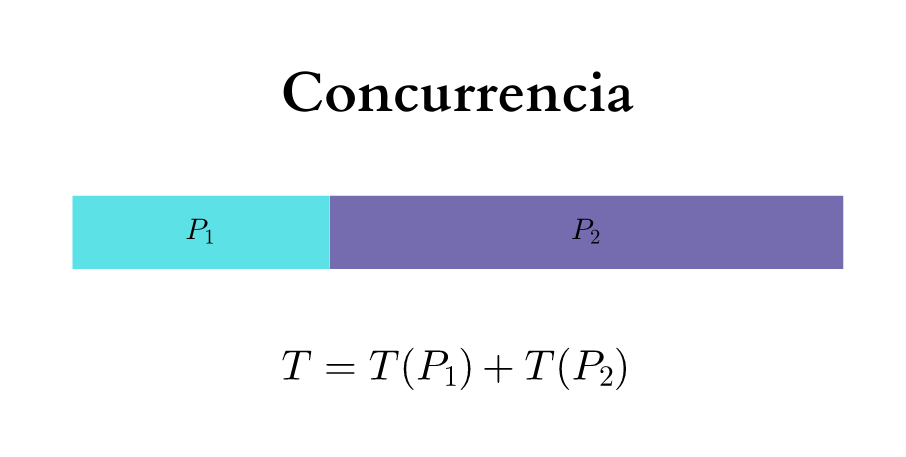
\includegraphics[width=5cm]{concurrencia.png}
	
	\imgcaption{1}{Tiempo de ejecuci\'on de programas concurrentes}
\end{center}

En el \textit{paralelismo} la ejecución ocurre en el mismo instante físico, los c\'alculos se realizan de forma verdaderamente simult\'anea. Para maximizar el uso de múltiples procesadores o n\'ucleos, presentes en las CPU modernas, el procesamiento en paralelo dividirá el trabajo entre varios subprocesos, cada uno de los cuales puede ejecutarse de forma independiente en un núcleo diferente. Paralelismo implica concurrencia, pero no se cumple el rec\'iproco. Sea ahora T el tiempo total de ejecuci\'on de dos programas paralelos $ P_{1} $ y $ P_{2} $:

\begin{center}
	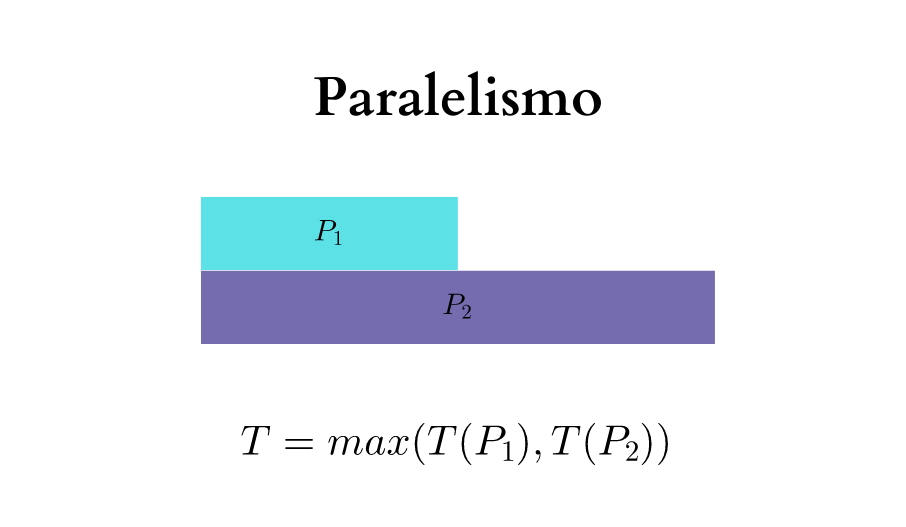
\includegraphics[width=5cm]{paralelismo.png}
	
	\imgcaption{2}{Tiempo de ejecuci\'on de programas paralelos}
\end{center}

En la programaci\'on concurrente ocurre con frecuencia que las hebras que se ejecuten necesiten sincronizar e intercambiar informaci\'on en alg\'un momento, lo cual se hace usualmente a trav\'es de memoria compartida. Esto puede causar problemas dado que varios procesos estar\'an realizando modificaciones concurrentemente sobre la misma memoria. M\'ultiples hebras se encuentran en una \textit{condici\'on de carrera} si el resultado de su ejecuci\'on depende del orden en que se ejecutan las instrucciones que componen cada hebra. 

Se denomina \textit{sección crítica} a la porción de código de una hebra en la que se accede a un recurso compartido y que puede entrar en una condici\'on de carrera, por lo que no debe ser accedido por más de un proceso o hilo en ejecución a la vez. Se necesita un mecanismo de sincronización en la entrada y salida de la sección crítica para asegurar la utilización exclusiva del recurso. Los recursos destinados a lograr este comportamiento se denominan de exclusi\'on mutua o \textit{mutex}. Los m\'as comunes son los candados, monitores y semáforos.

\subsection{Locks en C\#}

Los candados garantizan acceso exclusivo a un recurso compartido. La sincronizaci\'on se logra poni\'endole el candado a una variable. En C\# esto se logra mediante la palabra reservada \csl{lock}. 

El candado de exclusi\'on mutua es adquirido para un objeto dado por \csl{lock}, se ejecuta el bloque de c\'odigo dentro de su cuerpo y luego se libera el candado. Mientras un hilo mantenga un candado, este puede volver a adquirirlo y liberarlo. Cualquier otro subproceso no puede adquirir el candado y debe esperar hasta que este sea liberado. A continuaci\'on se muestra la forma de declarar un candado:

\begin{center}
	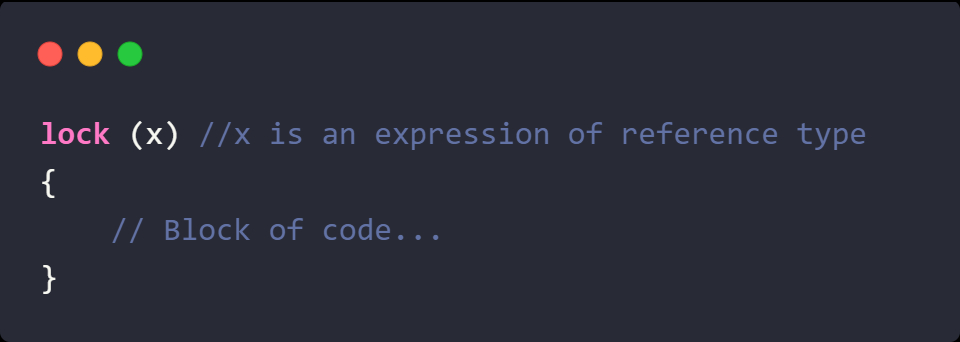
\includegraphics[width=8cm]{lock.jpg}
	
	\imgcaption{3}{Declaraci\'on de un candado}
\end{center}

\csl{lock} controla toda una secci\'on sin dejar libertad para adquirir o liberar un recurso basado en una l\'ogica m\'as propia del problema a solucionar. 

\subsection{Monitors en C\#}

Los monitores permiten sincronizar el acceso a una región de código tomando y liberando un bloqueo en un objeto en particular, de manera m\'as fluida que en los candados. En C\# se dispone de la clase \csl{System.Threading.Monitor} para este prop\'osito.

Un monitor se asocia a un objeto bajo demanda y se puede llamar directamente desde cualquier contexto. No se puede crear una instancia de esta clase. Sus métodos son todos estáticos y a cada uno se le pasa el objeto sincronizado que controla el acceso a la sección crítica.

Posee los m\'etodos \csl{Enter}, que adquiere un candado para un objeto y marca el comienzo de una sección crítica; y \csl{Exit}
que libera el bloqueo de un objeto, marcando el final de la sección crítica protegida por el objeto bloqueado. Se puede lograr entonces el comportamiento de un bloque \csl{lock} mediante un bloque \csl{try-finally} que utilice los m\'etodos \csl{Enter} y \csl{Exit} como se muestra a continuaci\'on:

\begin{center}
	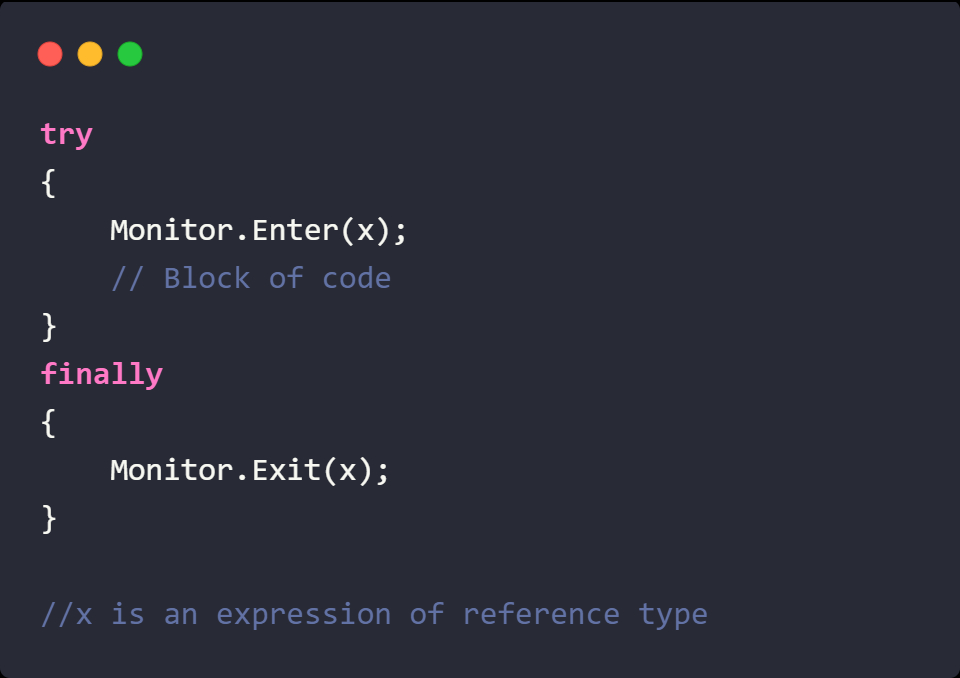
\includegraphics[width=8cm]{monitor.jpg} 
	
	\imgcaption{4}{Logrando comportamiento de candado con Monitors}
\end{center}

Adem\'as cuenta con los m\'etodos \csl{Wait} que libera el bloqueo de un objeto para permitir que otros subprocesos bloqueen y accedan al mismo; el subproceso que llama a este m\'etodo espera mientras otro subproceso accede al objeto; \csl{Pulse} y \csl{PulseAll}, quienes env\'ian una señal a los subprocesos en espera (uno y todos respectivamente), notific\'andoles que el estado del objeto bloqueado ha cambiado y que el propietario del bloqueo está listo para liberarlo. El subproceso en espera se coloca en la cola de subprocesos listos del objeto para que eventualmente pueda recibir el bloqueo para el mismo. 

\subsection{Semaphores en C\#}

Los sem\'aforos limitan la cantidad de subprocesos que pueden acceder a un recurso o conjunto de recursos al mismo tiempo. En C\# pueden ser encontrados en la clase \csl{System.Threading.Semaphore}.

Un sem\'aforo cuenta con dos propiedades fundamentales: \csl{Count}, que indica el n\'umero de hilos que pueden ingresar al sem\'aforo en este momento; y \csl{InitialCount}, que indica la cantidad m\'axima de hilos que pueden ingresar al sem\'aforo. Los subprocesos ingresan al semáforo llamando al método \csl{WaitOne()}, y liberan el semáforo llamando al método \csl{Release()}.

El \csl{Count} en un semáforo se reduce cada vez que un subproceso ingresa al semáforo y se incrementa cuando un subproceso libera el semáforo. Cuando el \csl{Count} es cero, las solicitudes posteriores se bloquean hasta que otros subprocesos liberan el semáforo; no hay un orden predeterminado en el que los subprocesos bloqueados entren en el semáforo. Cuando todos los subprocesos han liberado el semáforo, el \csl{Count} estar\'a en el valor máximo especificado cuando se creó el semáforo (\csl{InitialCount}).

Un subproceso puede ingresar el semáforo varias veces llamando al método \csl{WaitOne()} repetidamente. Para liberar algunas o todas estas entradas, el subproceso puede llamar a la sobrecarga del método \csl{Release()} sin parámetros varias veces, o puede llamar a la sobrecarga del método \csl{Release(int)} que especifica la cantidad de entradas que se liberarán. No se aplica la identidad del subproceso en las llamadas a \csl{WaitOne()} o \csl{Release()}, por lo que es responsabilidad del programador asegurarse de que los subprocesos no liberen el semáforo m\'as veces de las requeridas. Esto es importante pues si, por ejemplo, un semáforo tiene un recuento máximo de dos y tanto el hilo A como el hilo B entran en el semáforo, si un error de programación en el subproceso B hace que llame a \csl{Release} dos veces, ambas llamadas se realizan correctamente. El conteo en el semáforo estar\'a lleno, y cuando el subproceso A eventualmente llame a \csl{Release}, se lanzar\'a una excepci\'on \csl{SemaphoreFullException}.

Un sem\'aforo puede ser de dos tipos: local o nombrado del sistema. Un semáforo local existe solo dentro de su proceso, pudiendo ser utilizado por cualquier subproceso en este que tenga una referencia al mismo. Por otro lado, si se crea un sem\'aforo utilizando un constructor que acepta un nombre, se asocia con un semáforo del sistema operativo de ese nombre, siendo visible en todo el sistema operativo y pudiendo utilizarse para sincronizar las actividades de los procesos. Se puede usar el método \csl{OpenExisting} para abrir un semáforo nombrado del sistema existente.

En la figura siguiente se muestra una implementación de la clase Semaphore en C\# usando la clase Monitor:

\begin{center}
	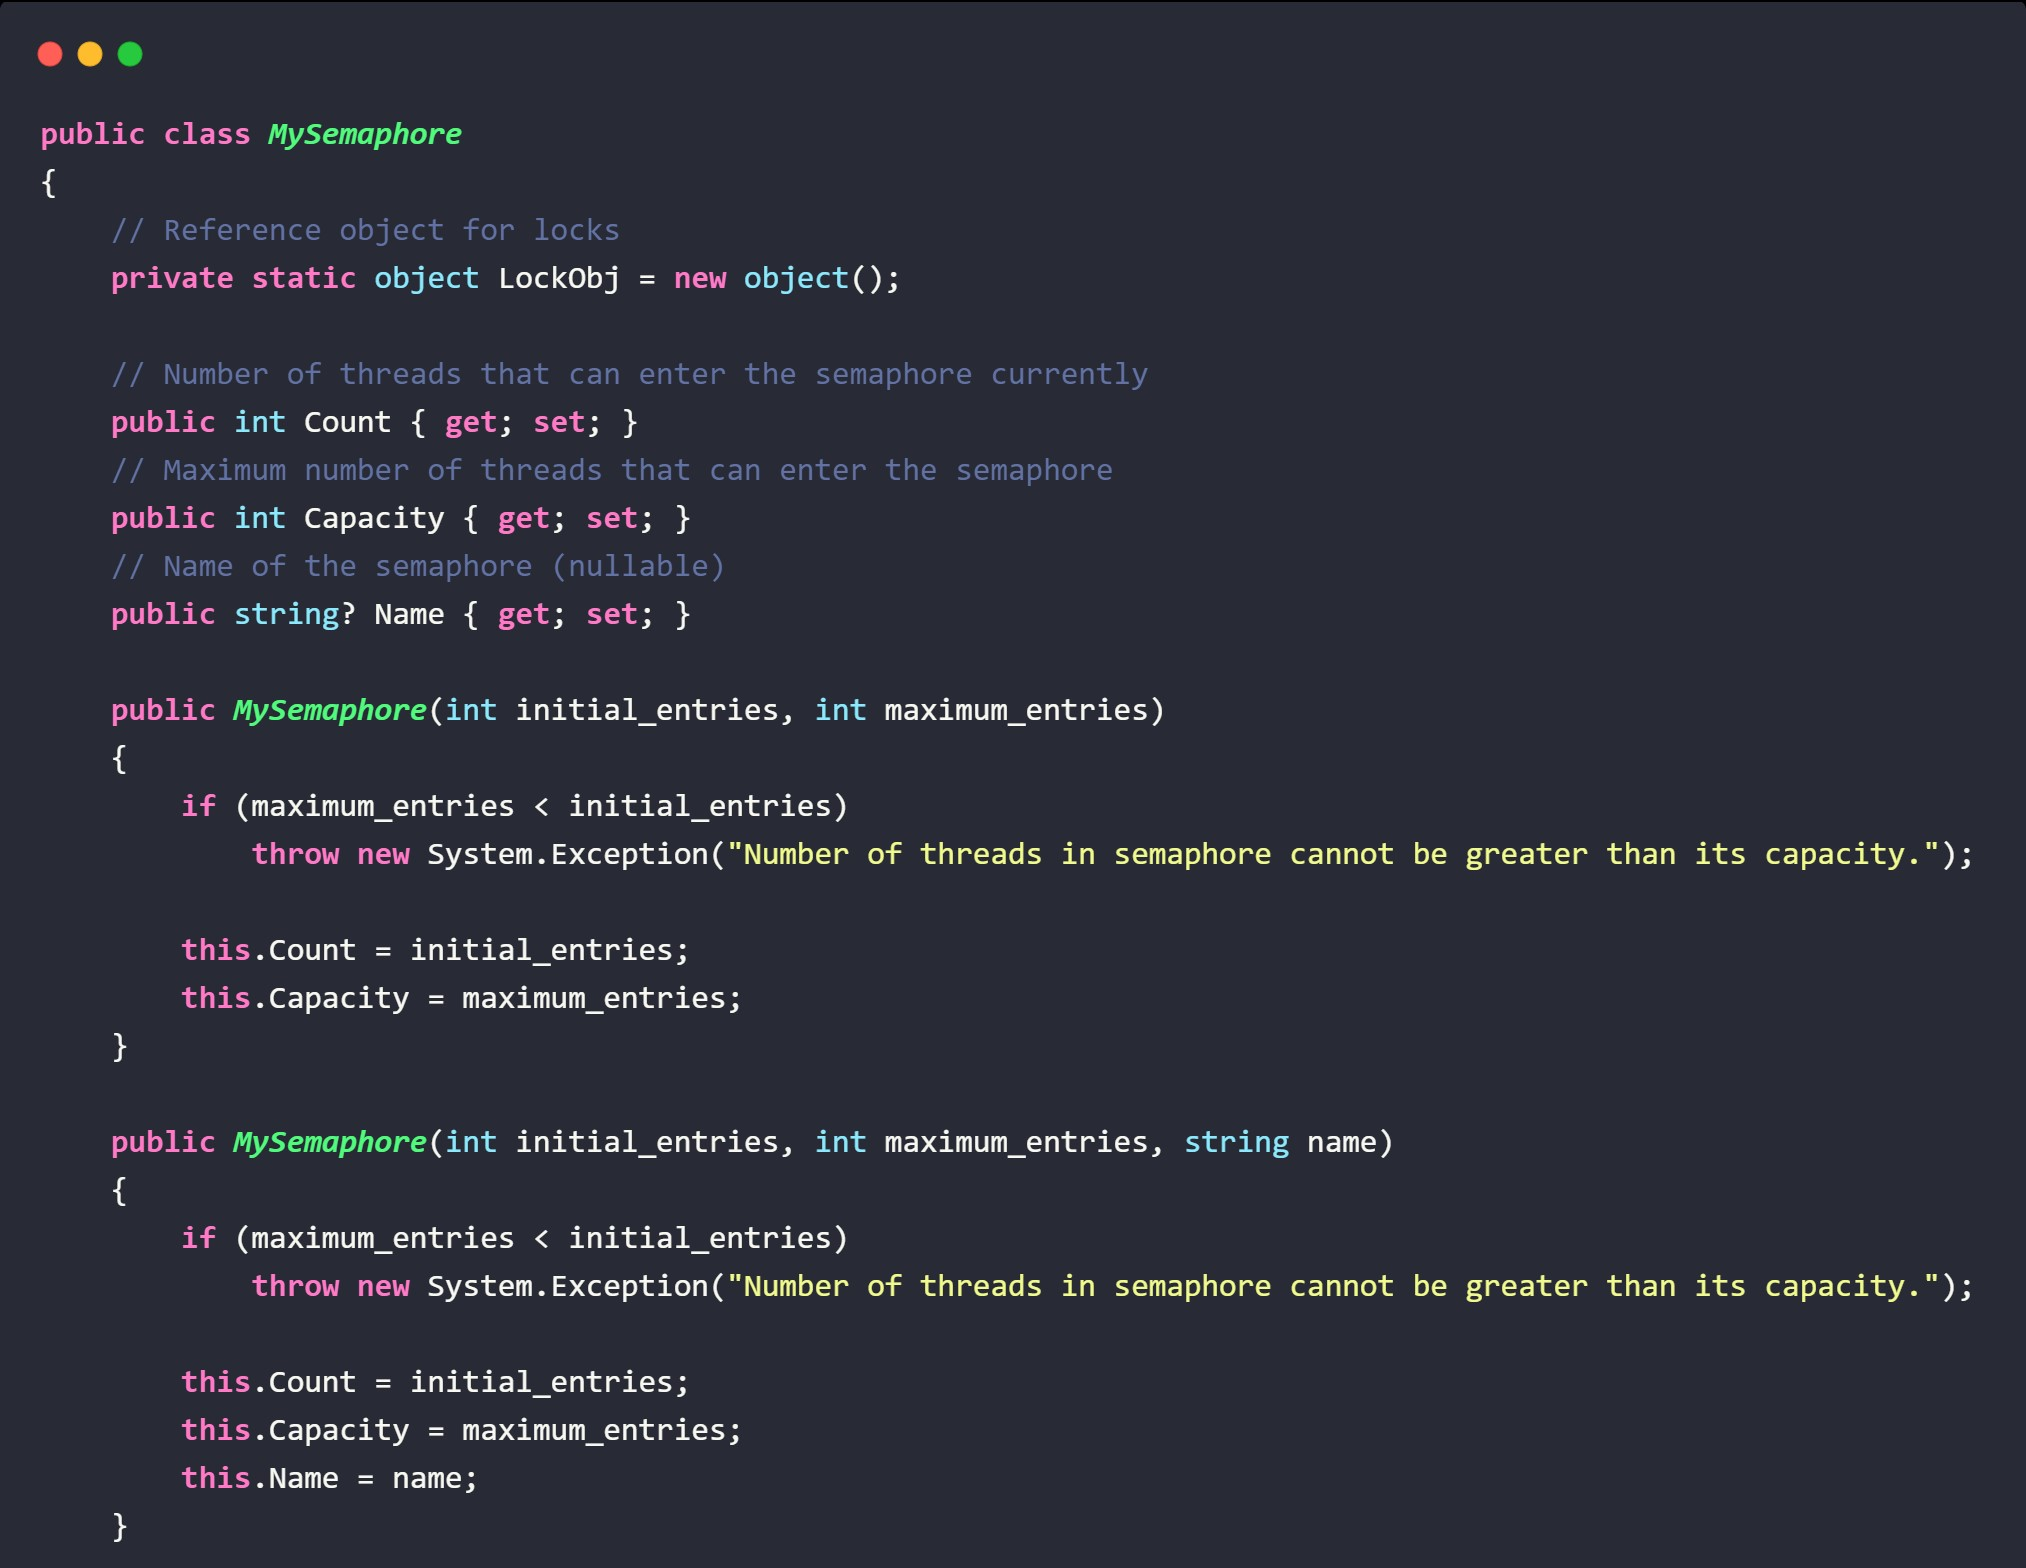
\includegraphics[width=15cm]{MySemaphore1.jpg}
\end{center}

\begin{center}
	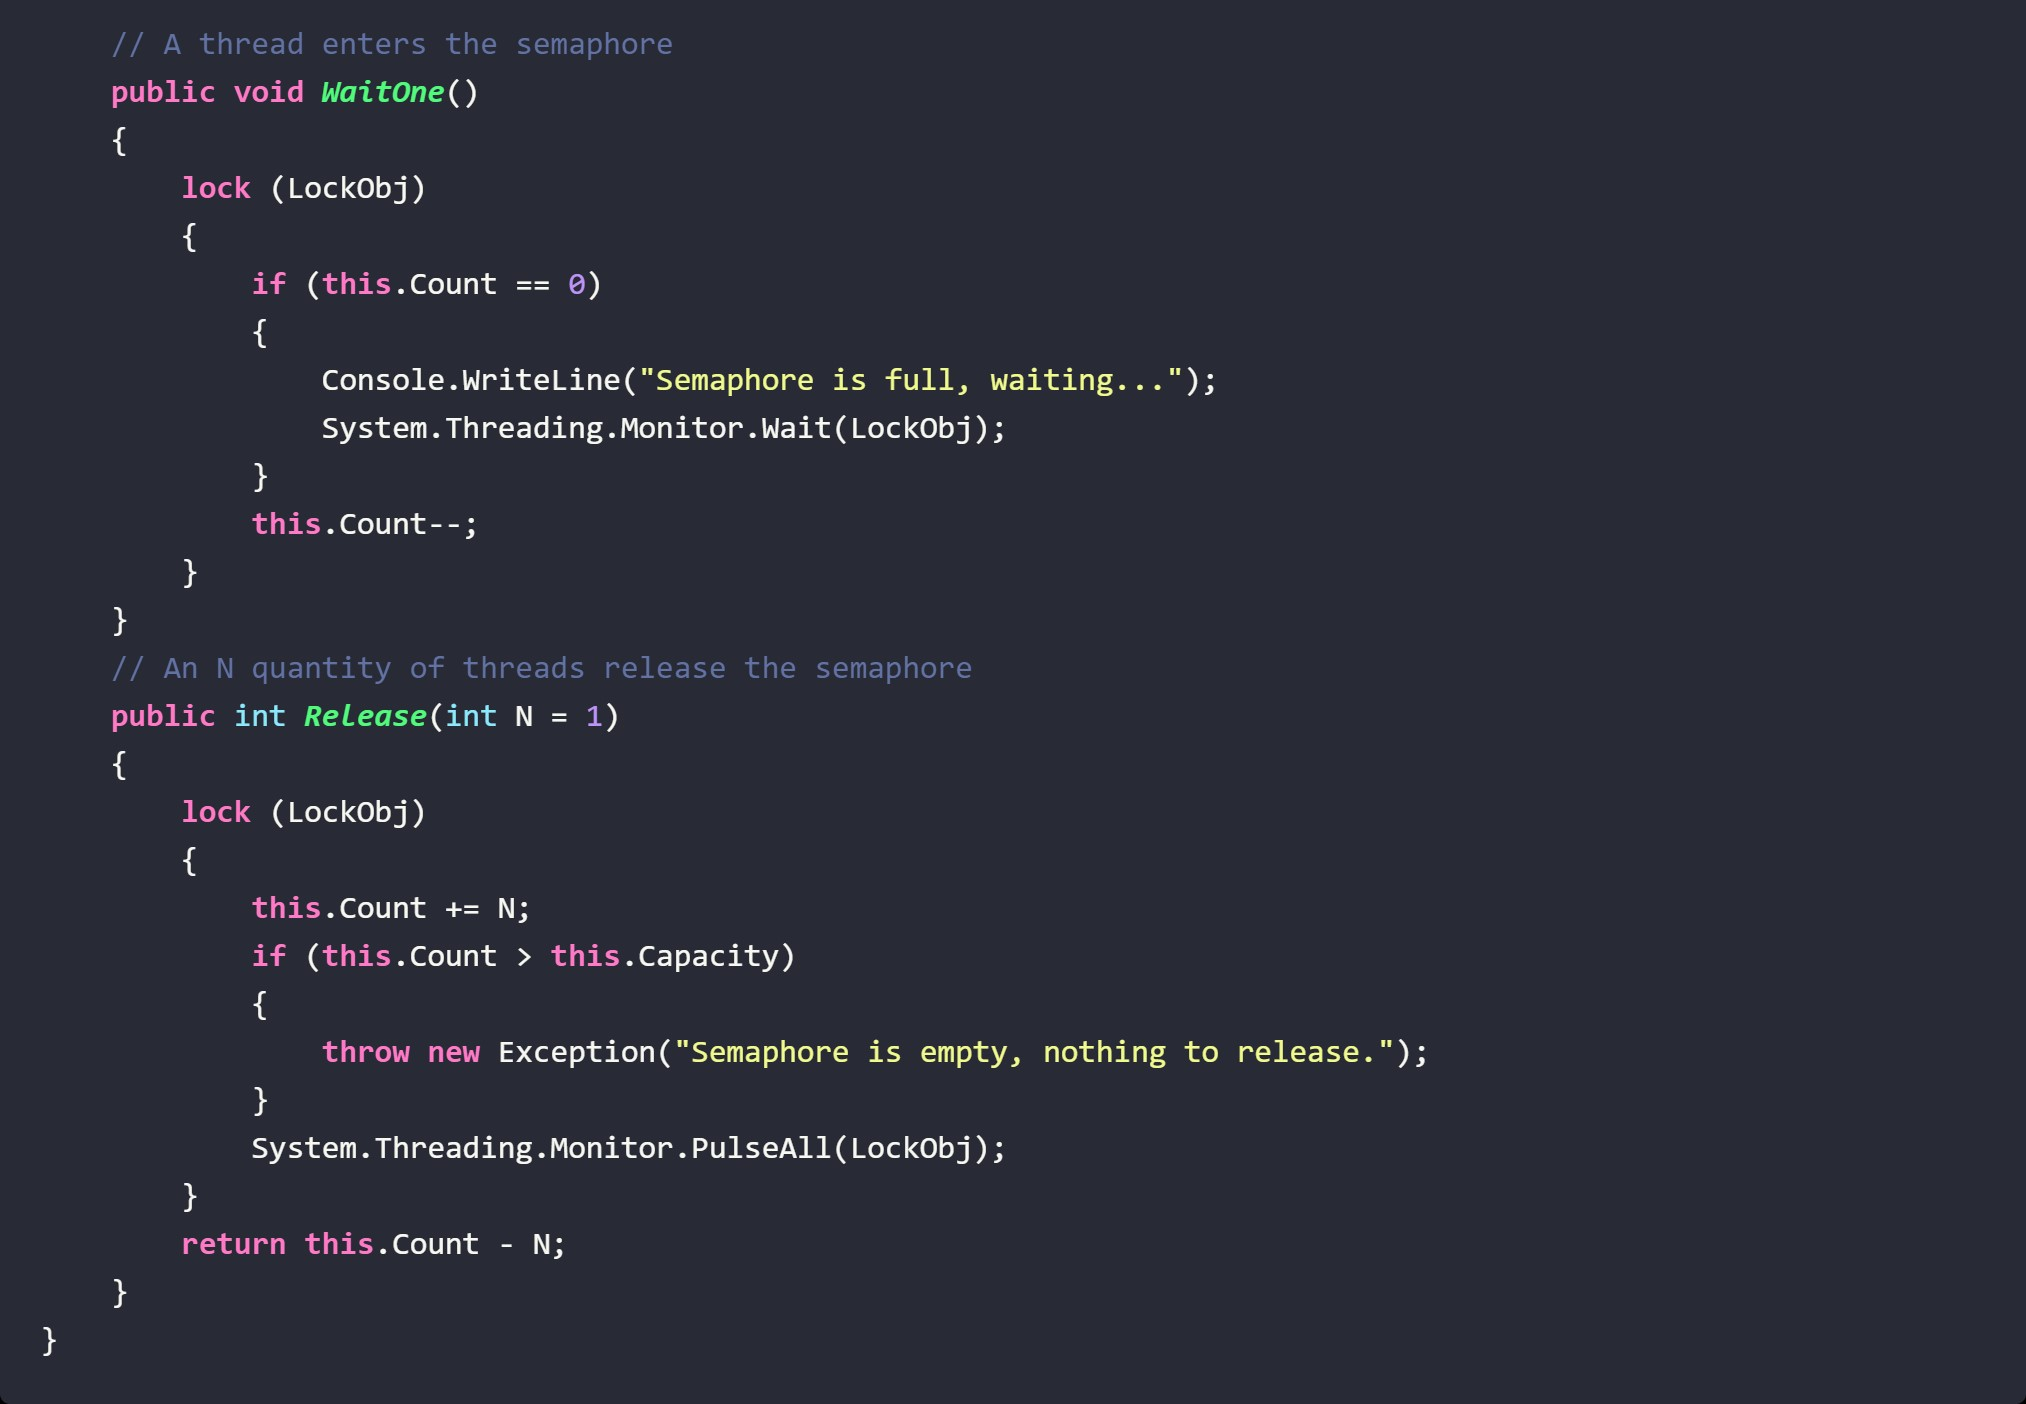
\includegraphics[width=15cm]{MySemaphore2.jpg}
	
	\imgcaption{5}{Implementaci\'on de MySemaphore utilizando Monitors}
\end{center}

\subsection{Barriers en C\#}

Permite que múltiples tareas trabajen de manera cooperativa en un algoritmo en paralelo a través de múltiples fases. Ninguna hebra puede comenzar una nueva fase del algoritmo hasta que las restantes hebras no hayan alcanzado la barrera (todas hallan completado la fase anterior).

El constructor m\'as simple de la clase toma por argumento un entero, que representar\'a el m\'aximo n\'umero de participantes (hilos) que pueden estar esperando por la barrera en cada fase del algoritmo. Los m\'etodos \csl{AddParticipant()} y \csl{RemoveParticipant()} permiten aumentar en una unidad la cantidad m\'axima de participantes. 

El m\'etodo fundamental de la clase es \csl{SignalAndWait()}. Este es invocado por una hebra cuando llega a un punto en que est\'a lista para moverse a la siguiente fase. Este advierte a la instancia de \emph{Barrier} de que un nuevo participante ha llegado a la barrera. Cuando hayan llegado una cantidad de participantes igual al n\'umero m\'aximo entonces la barrera entra en la post-phase. Aqu\'i es donde incrementa el n\'umero de la fase, y le da la se\~nal a todos los participantes de que pueden entrar en la nueva fase. Adicionalmente mediante el otro constructor de Barrier se puede establecer una acci\'on que se ejecutar\'a en cada post-phase. 

El \'ultimo m\'etodo relevante que posee es el \csl{Dispose()} que permite liberar los recursos usados por la barrera cuando esta no se necesite usar m\'as. Si se intenta usar la barrera despu\'es de que esta haya sido ``disposed", lanzar\'a una excepci\'on del tipo \emph{ObjectDisposedException}. Los otros tipos de excepciones lanzadas por los m\'etodos de la clase son \emph{InvalidOperationException} y \emph{BarrierPostPhaseException}. La primera de estas ocurre cuando en la barrera est\'an esperando m\'as participantes que el m\'aximo permitido o cuando se invoca alguno de sus m\'etodos estando en la post-phase. La segunda ocurre cuando la acci\'on establecida a ejecutar entre fases lanza una excepci\'on. Esta es capturada y envuelta (wrapped) en una excepci\'on del tipo mencionada y relanzada en cada uno de los hilos (participantes).

Para implementar la clase Barrier se hizo uso de la clase \csl{Monitor}. Para ello en el cuerpo del m\'etodo \csl{SignalAndWait()} se usa \csl{Monitor.Wait} para hacer que la hebra que lo ejecuta espere a que el resto llegue a la barrera. Cada vez que llega una hebra nueva se incrementa la cantidad de participantes que han llegado. Cuando se alcanza el m\'aximo lo primero que se ejecuta la acci\'on prefijada (si alguna), desde la \'ultima hebra en llegar. Entonces se incrementa el n\'umero de la fase y se invoca \csl{Monitor.PulseAll} para que todas las hebras reanuden su ejecuci\'on. Sin embargo, se tuvo mucha sutileza para manejar la mayor cantidad de casos posibles en que pudieran ocurrir errores de sincronizaci\'on, como podr\'ia ser la muerte por inanici\'on. Se maneja cada situaci\'on de la manera m\'as correcta posible seg\'un criterio de los autores, y se lanza la excepci\'on adecuada en cada caso, seg\'un lo descrito sobre estas anteriormente.

\begin{center}
	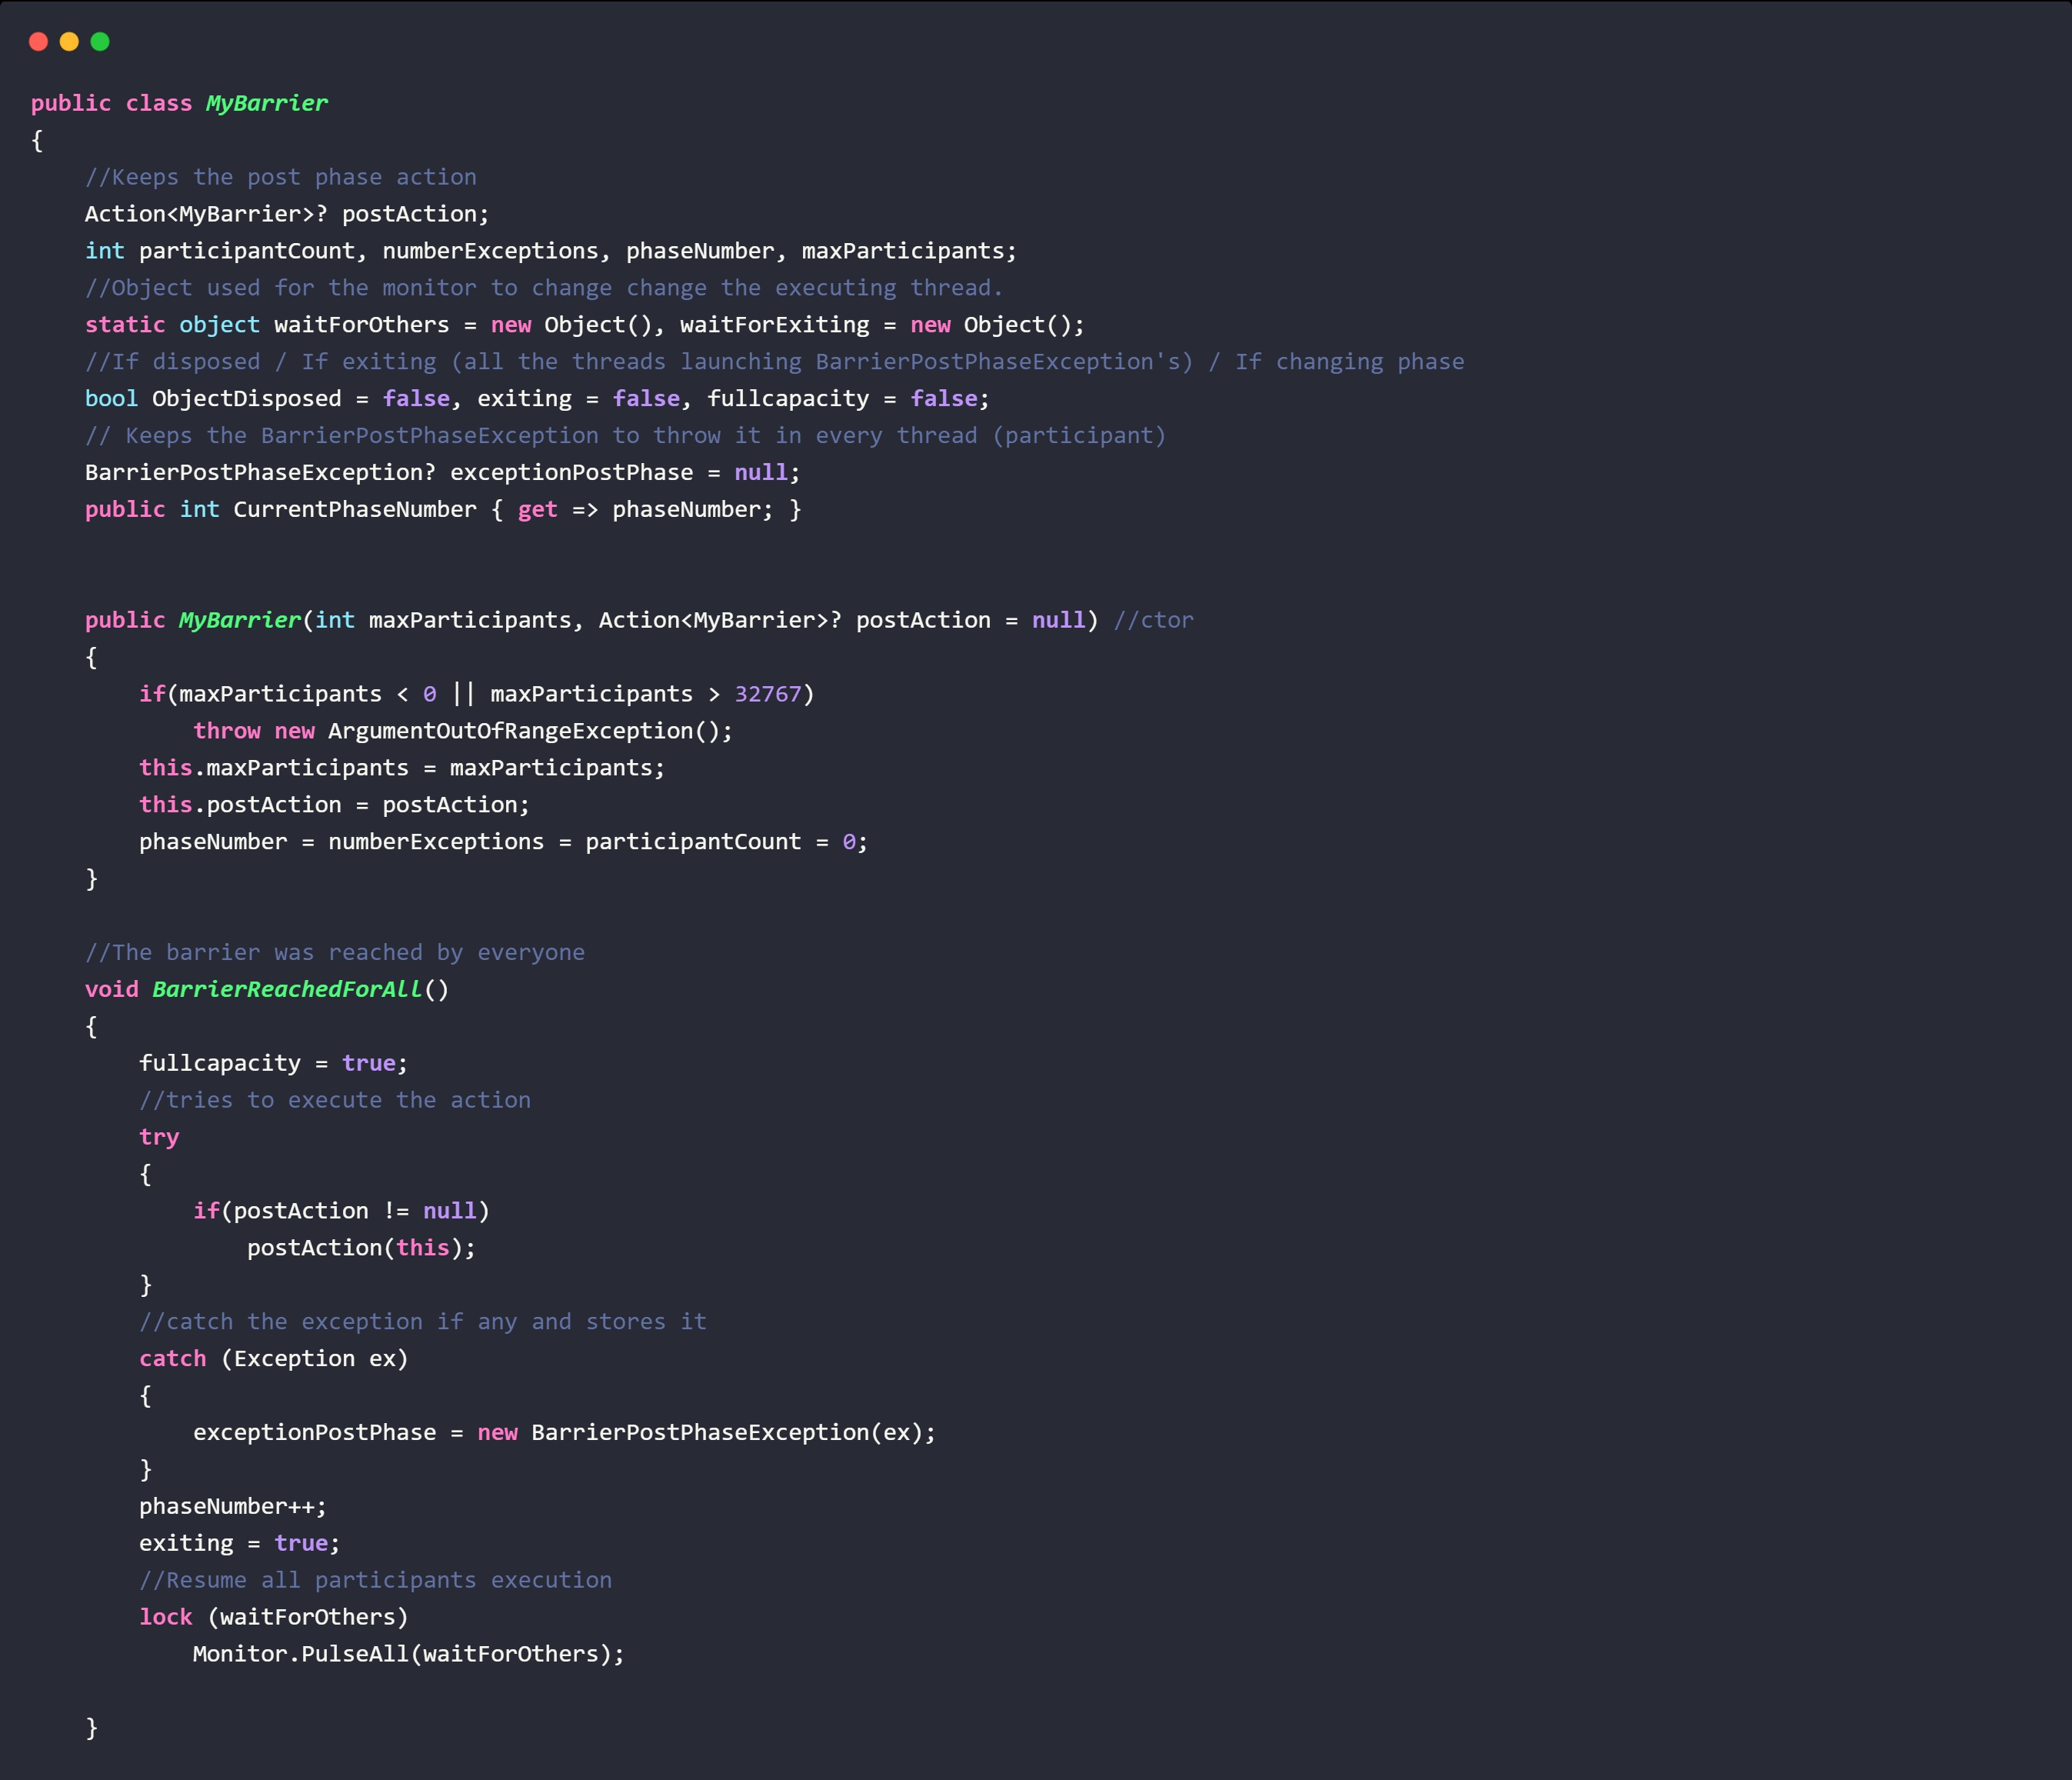
\includegraphics[width=15cm]{MyBarrier1.jpg}
\end{center}

\begin{center}
	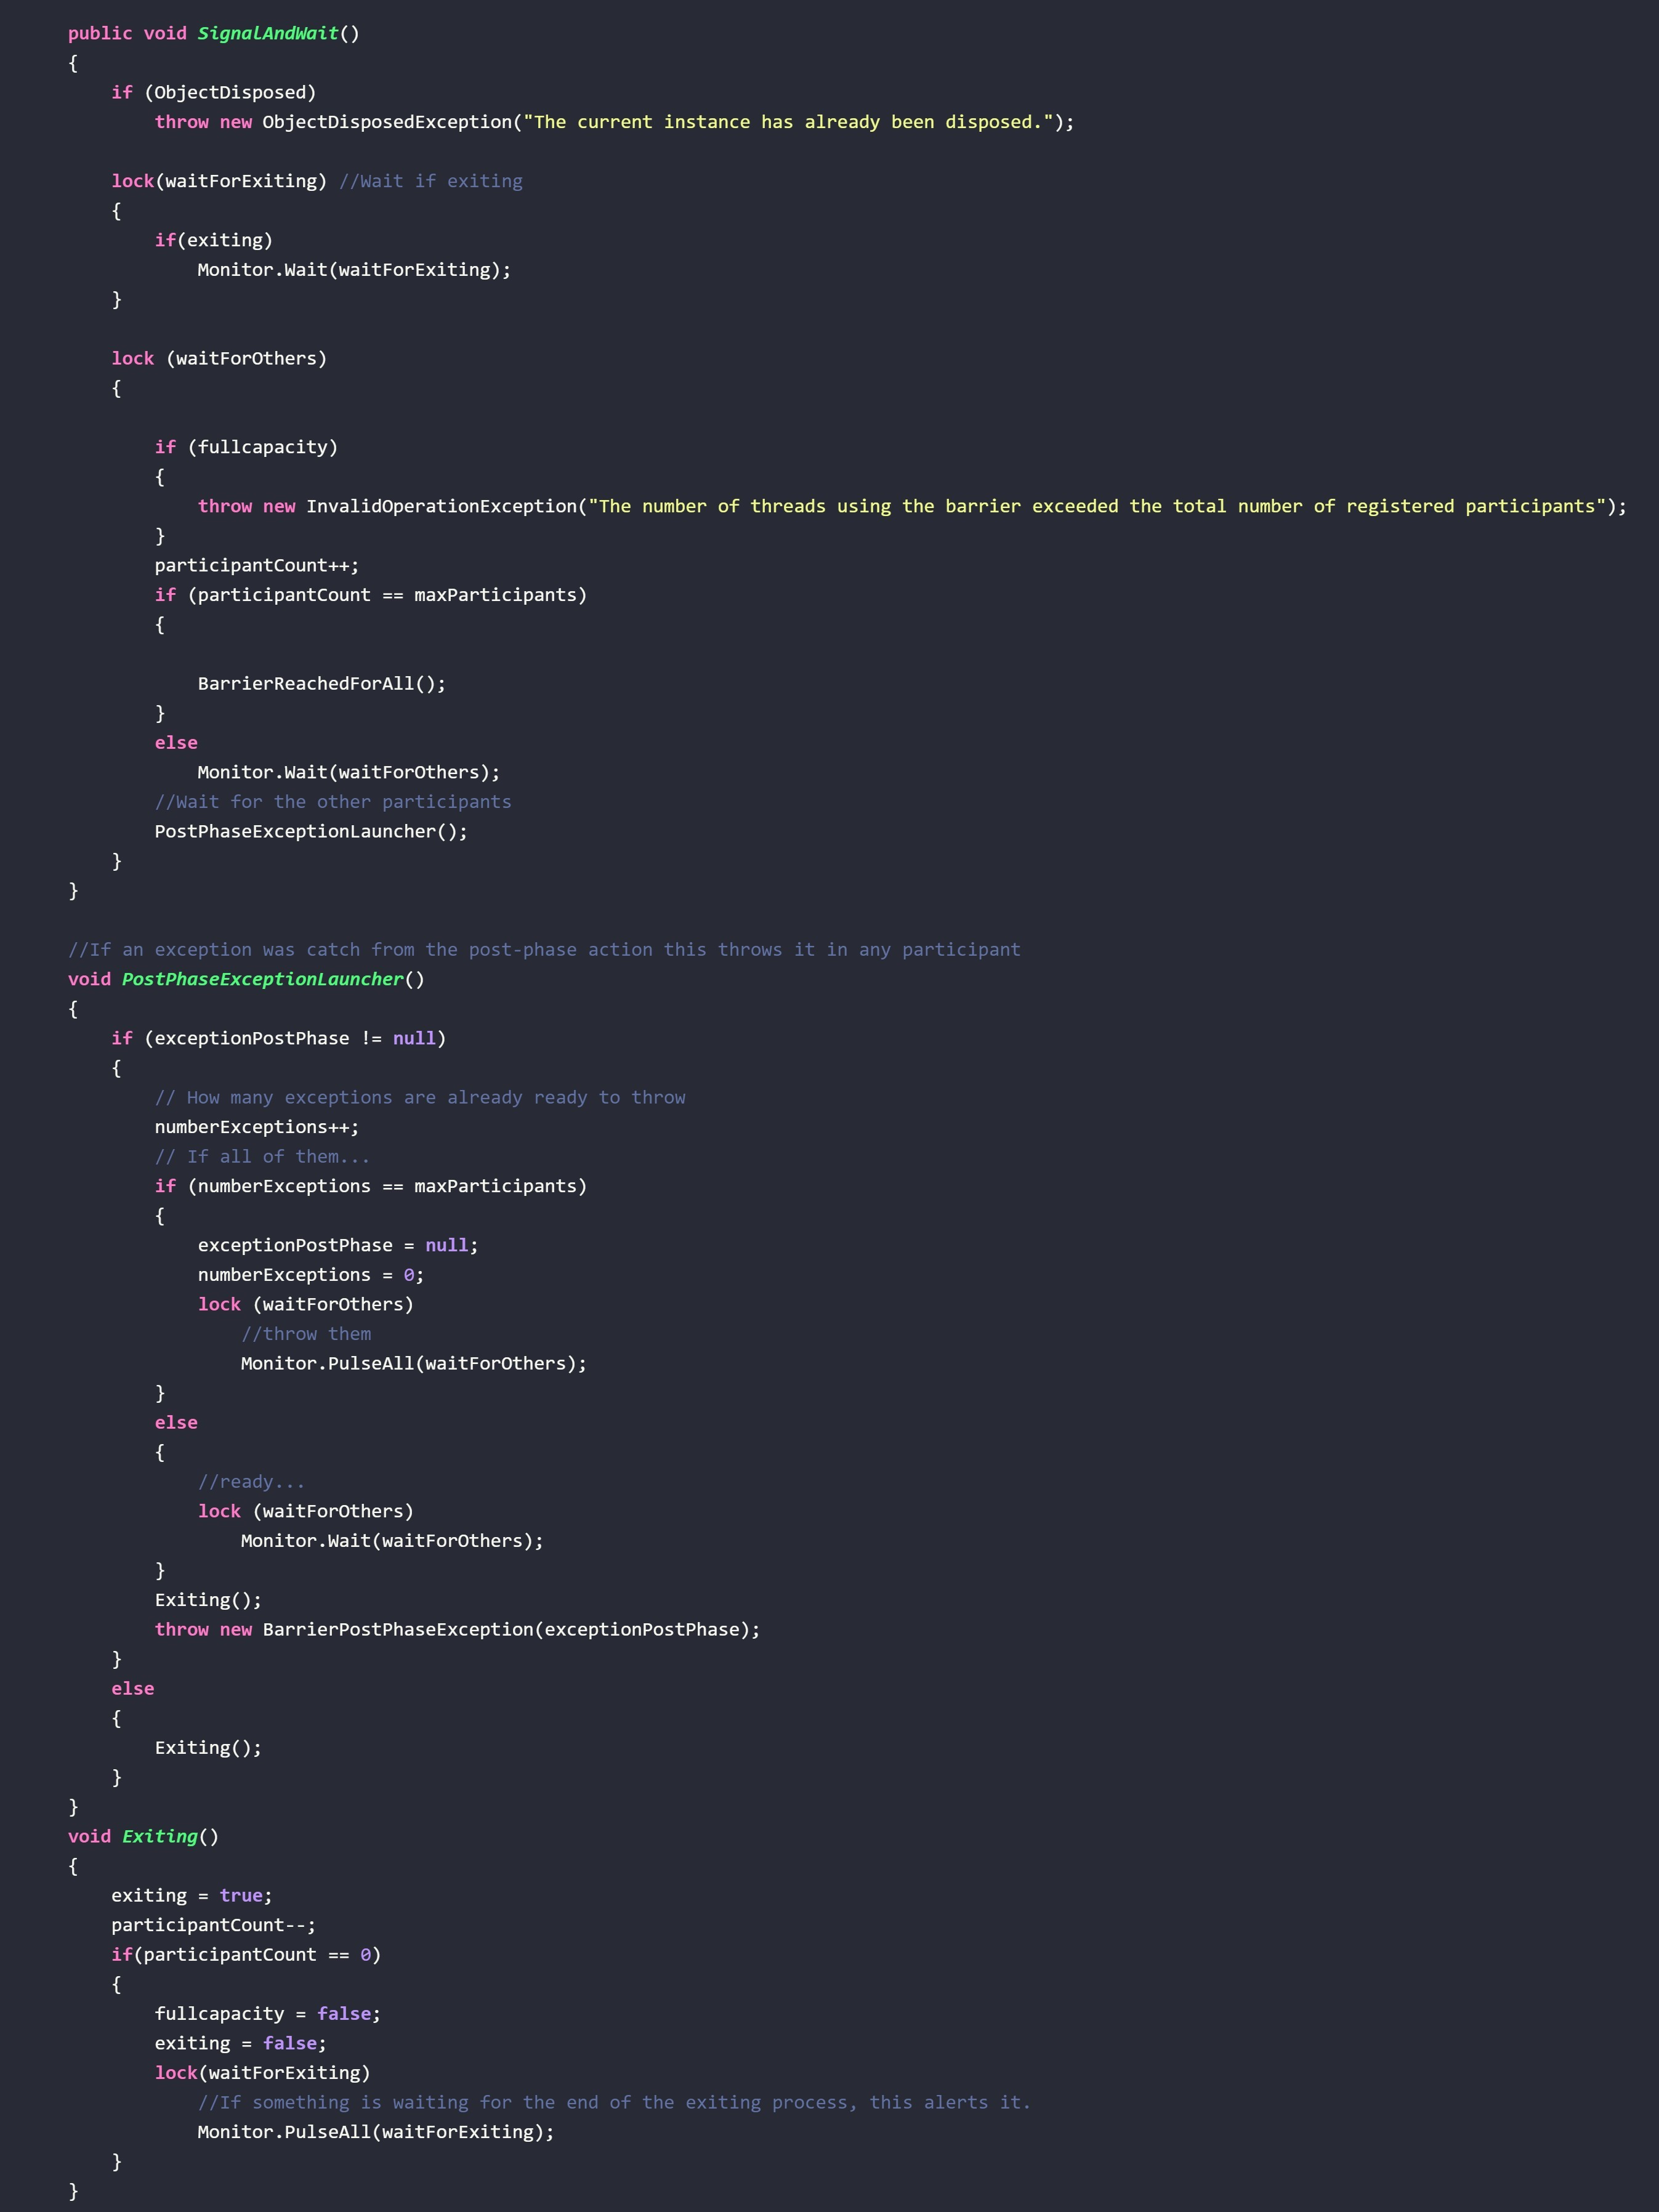
\includegraphics[width=15cm]{MyBarrier2.jpg}
\end{center}

\begin{center}
	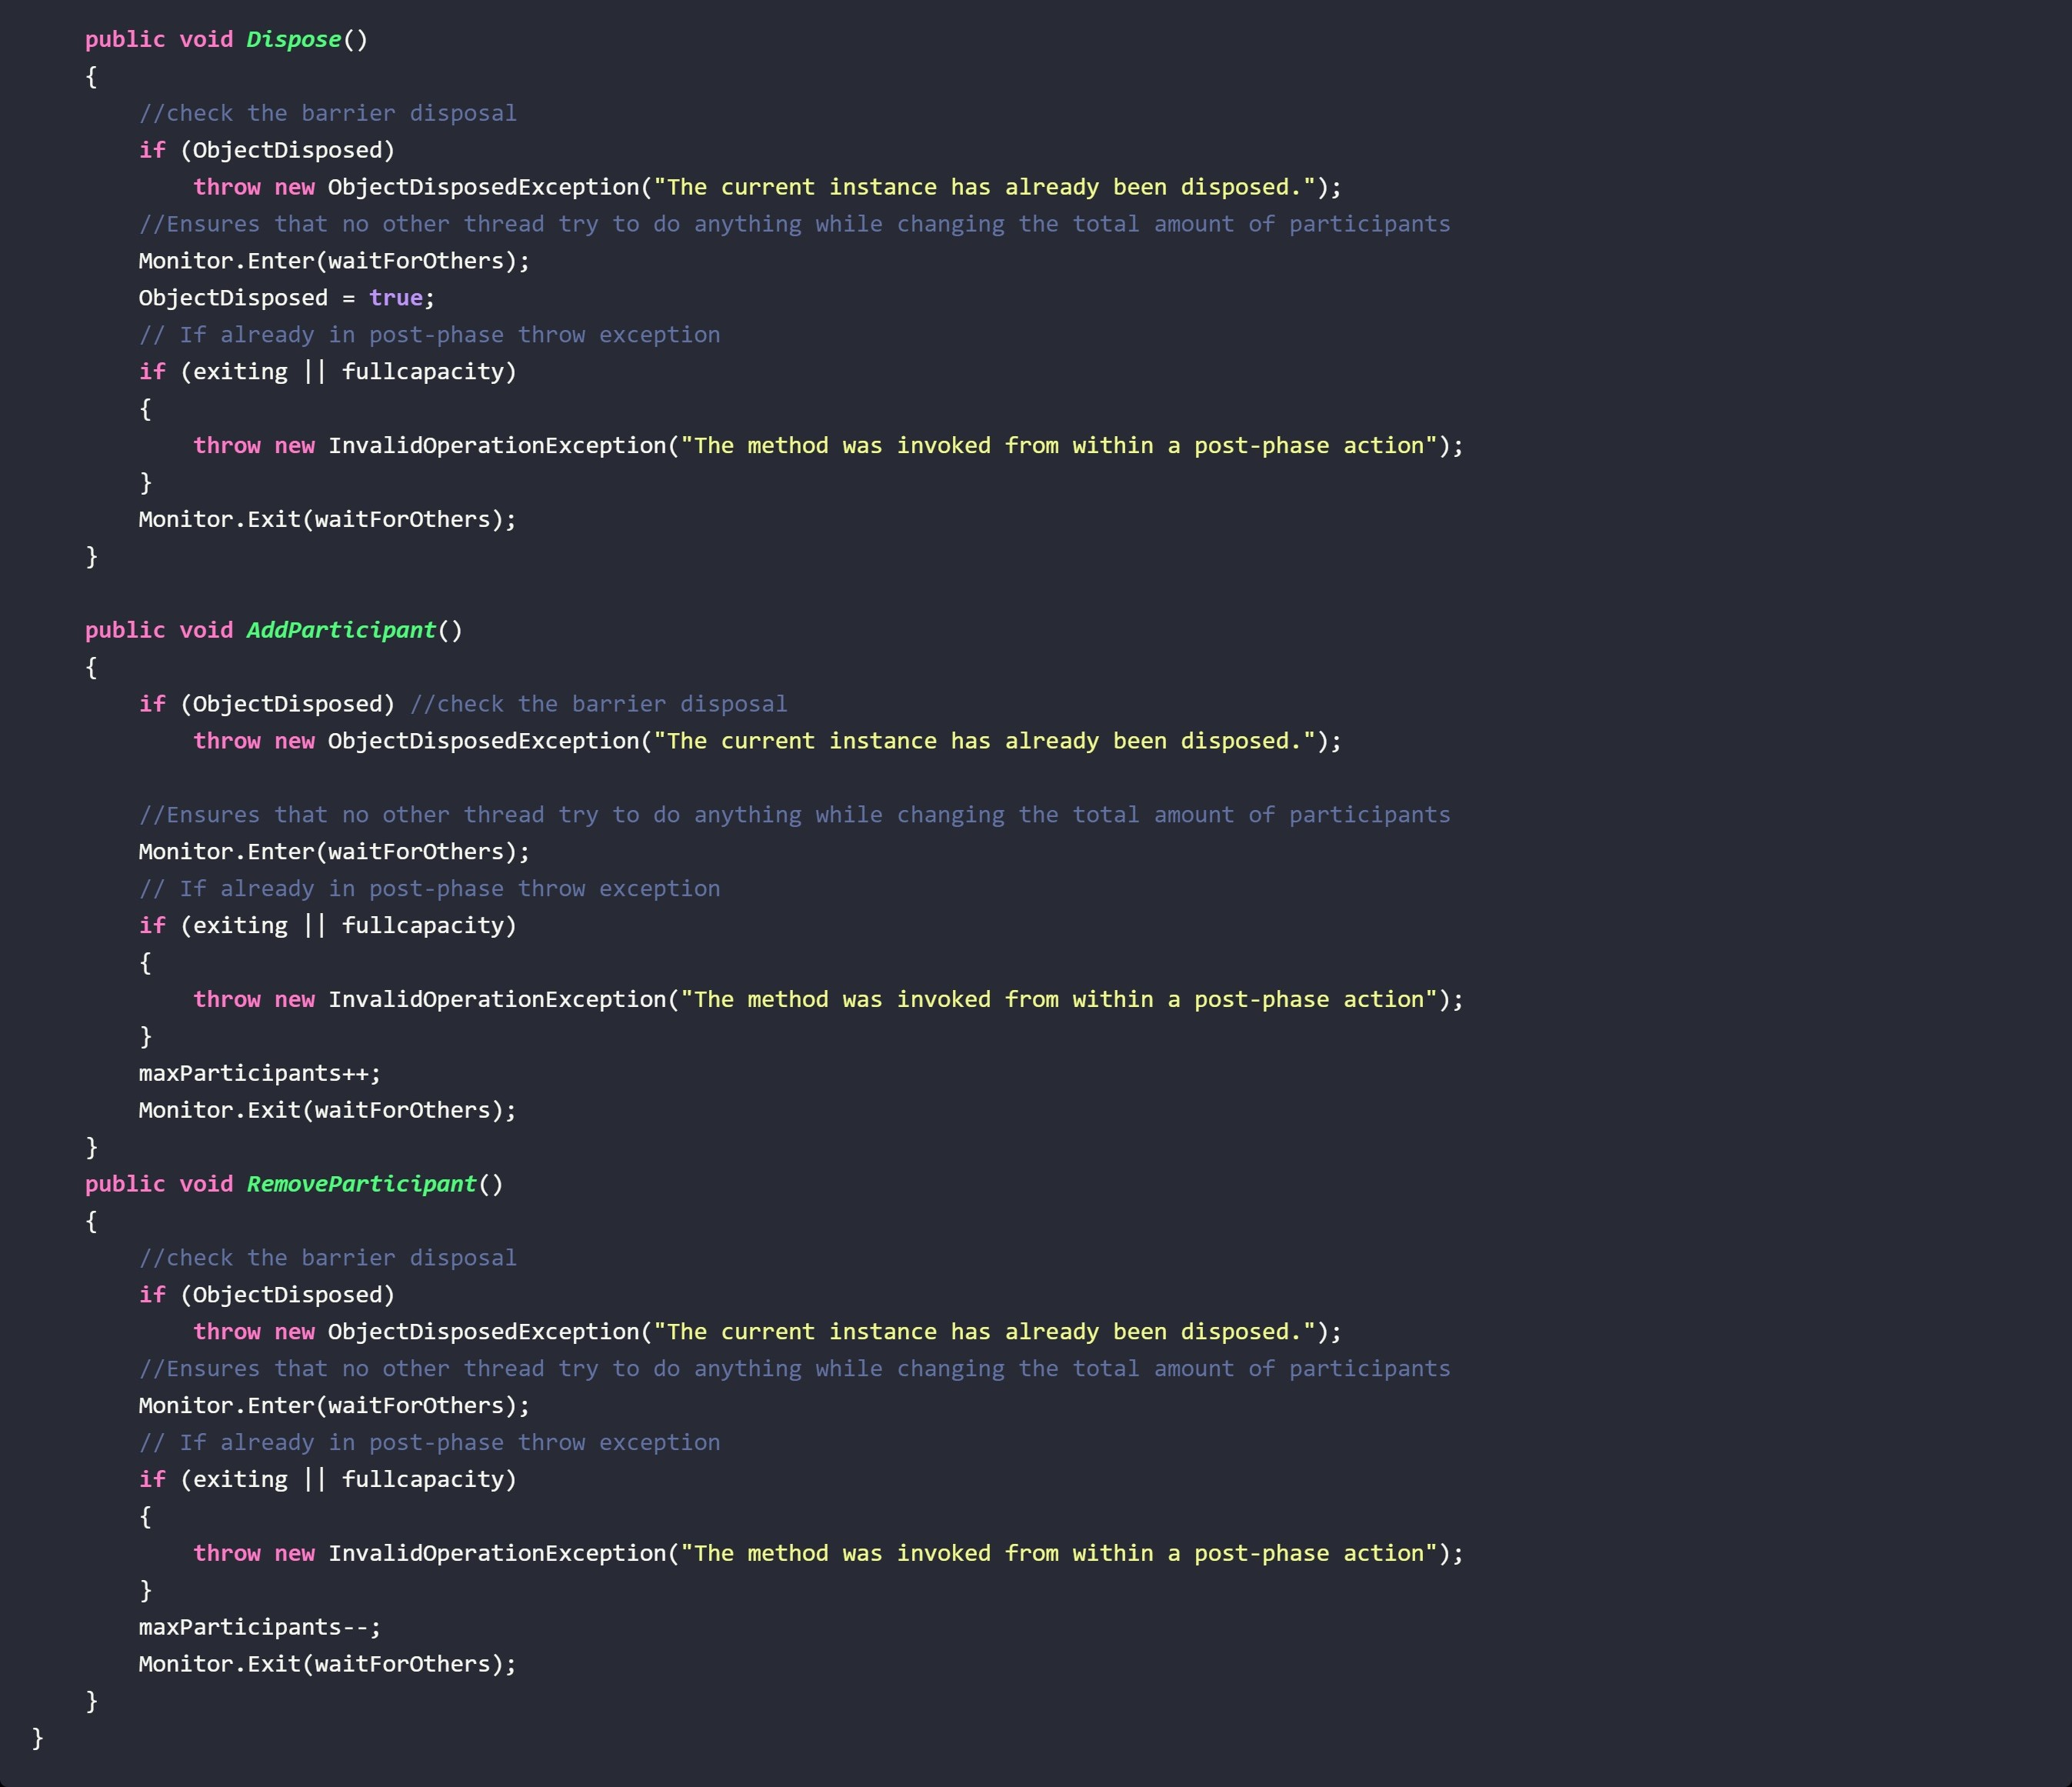
\includegraphics[width=15cm]{MyBarrier3.jpg}
	
	\imgcaption{6}{Implementaci\'on de MyBarrier utilizando Monitors}
\end{center}

\subsection{Countdowns en C\#}

Los countdowns permiten sincronizar ejecuciones de m\'ultiples hebras mediante cuentas regresivas. Dado el n\'umero de eventos que tienen que ocurrir para realizar una acci\'on, se notifica cada vez que termine uno de estos eventos disminuyendo el contador, y se emite una se\~nal cuando la cuenta llegue a cero. En C\# esta funcionalidad se implementa con la clase \csl{System.Threading.CountdownEvent}. 

Cuenta con distintas propiedades: \csl{CurrentCount} que obtiene el número de señales restantes necesarias para establecer el evento, \csl{InitialCount} que obtiene el número de señales requeridas inicialmente para configurar el evento, y \csl{IsSet} que indica si el recuento actual del objeto \csl{CountdownEvent} ha llegado a cero, para emitir la se\~nal.
	
Sus m\'etodos fundamentales son \csl{AddCount(Int32)} que incrementa el recuento actual de \csl{CountdownEvent} en un valor especificado, \csl{Reset(Int32)} que restablece la propiedad \csl{InitialCount} a un valor especificado, \csl{Signal(Int32)} quien registra múltiples señales con \csl{CountdownEvent}, disminuyendo el valor de \csl{CurrentCount} en la cantidad especificada, y \csl{Wait()}, encargado de bloquear el subproceso actual hasta que se establece \csl{CountdownEvent}.

En la figura siguiente se muestra una implementación de la clase \csl{CountdownEvent} en C\# usando la clase \csl{Monitor}:

\begin{center}
	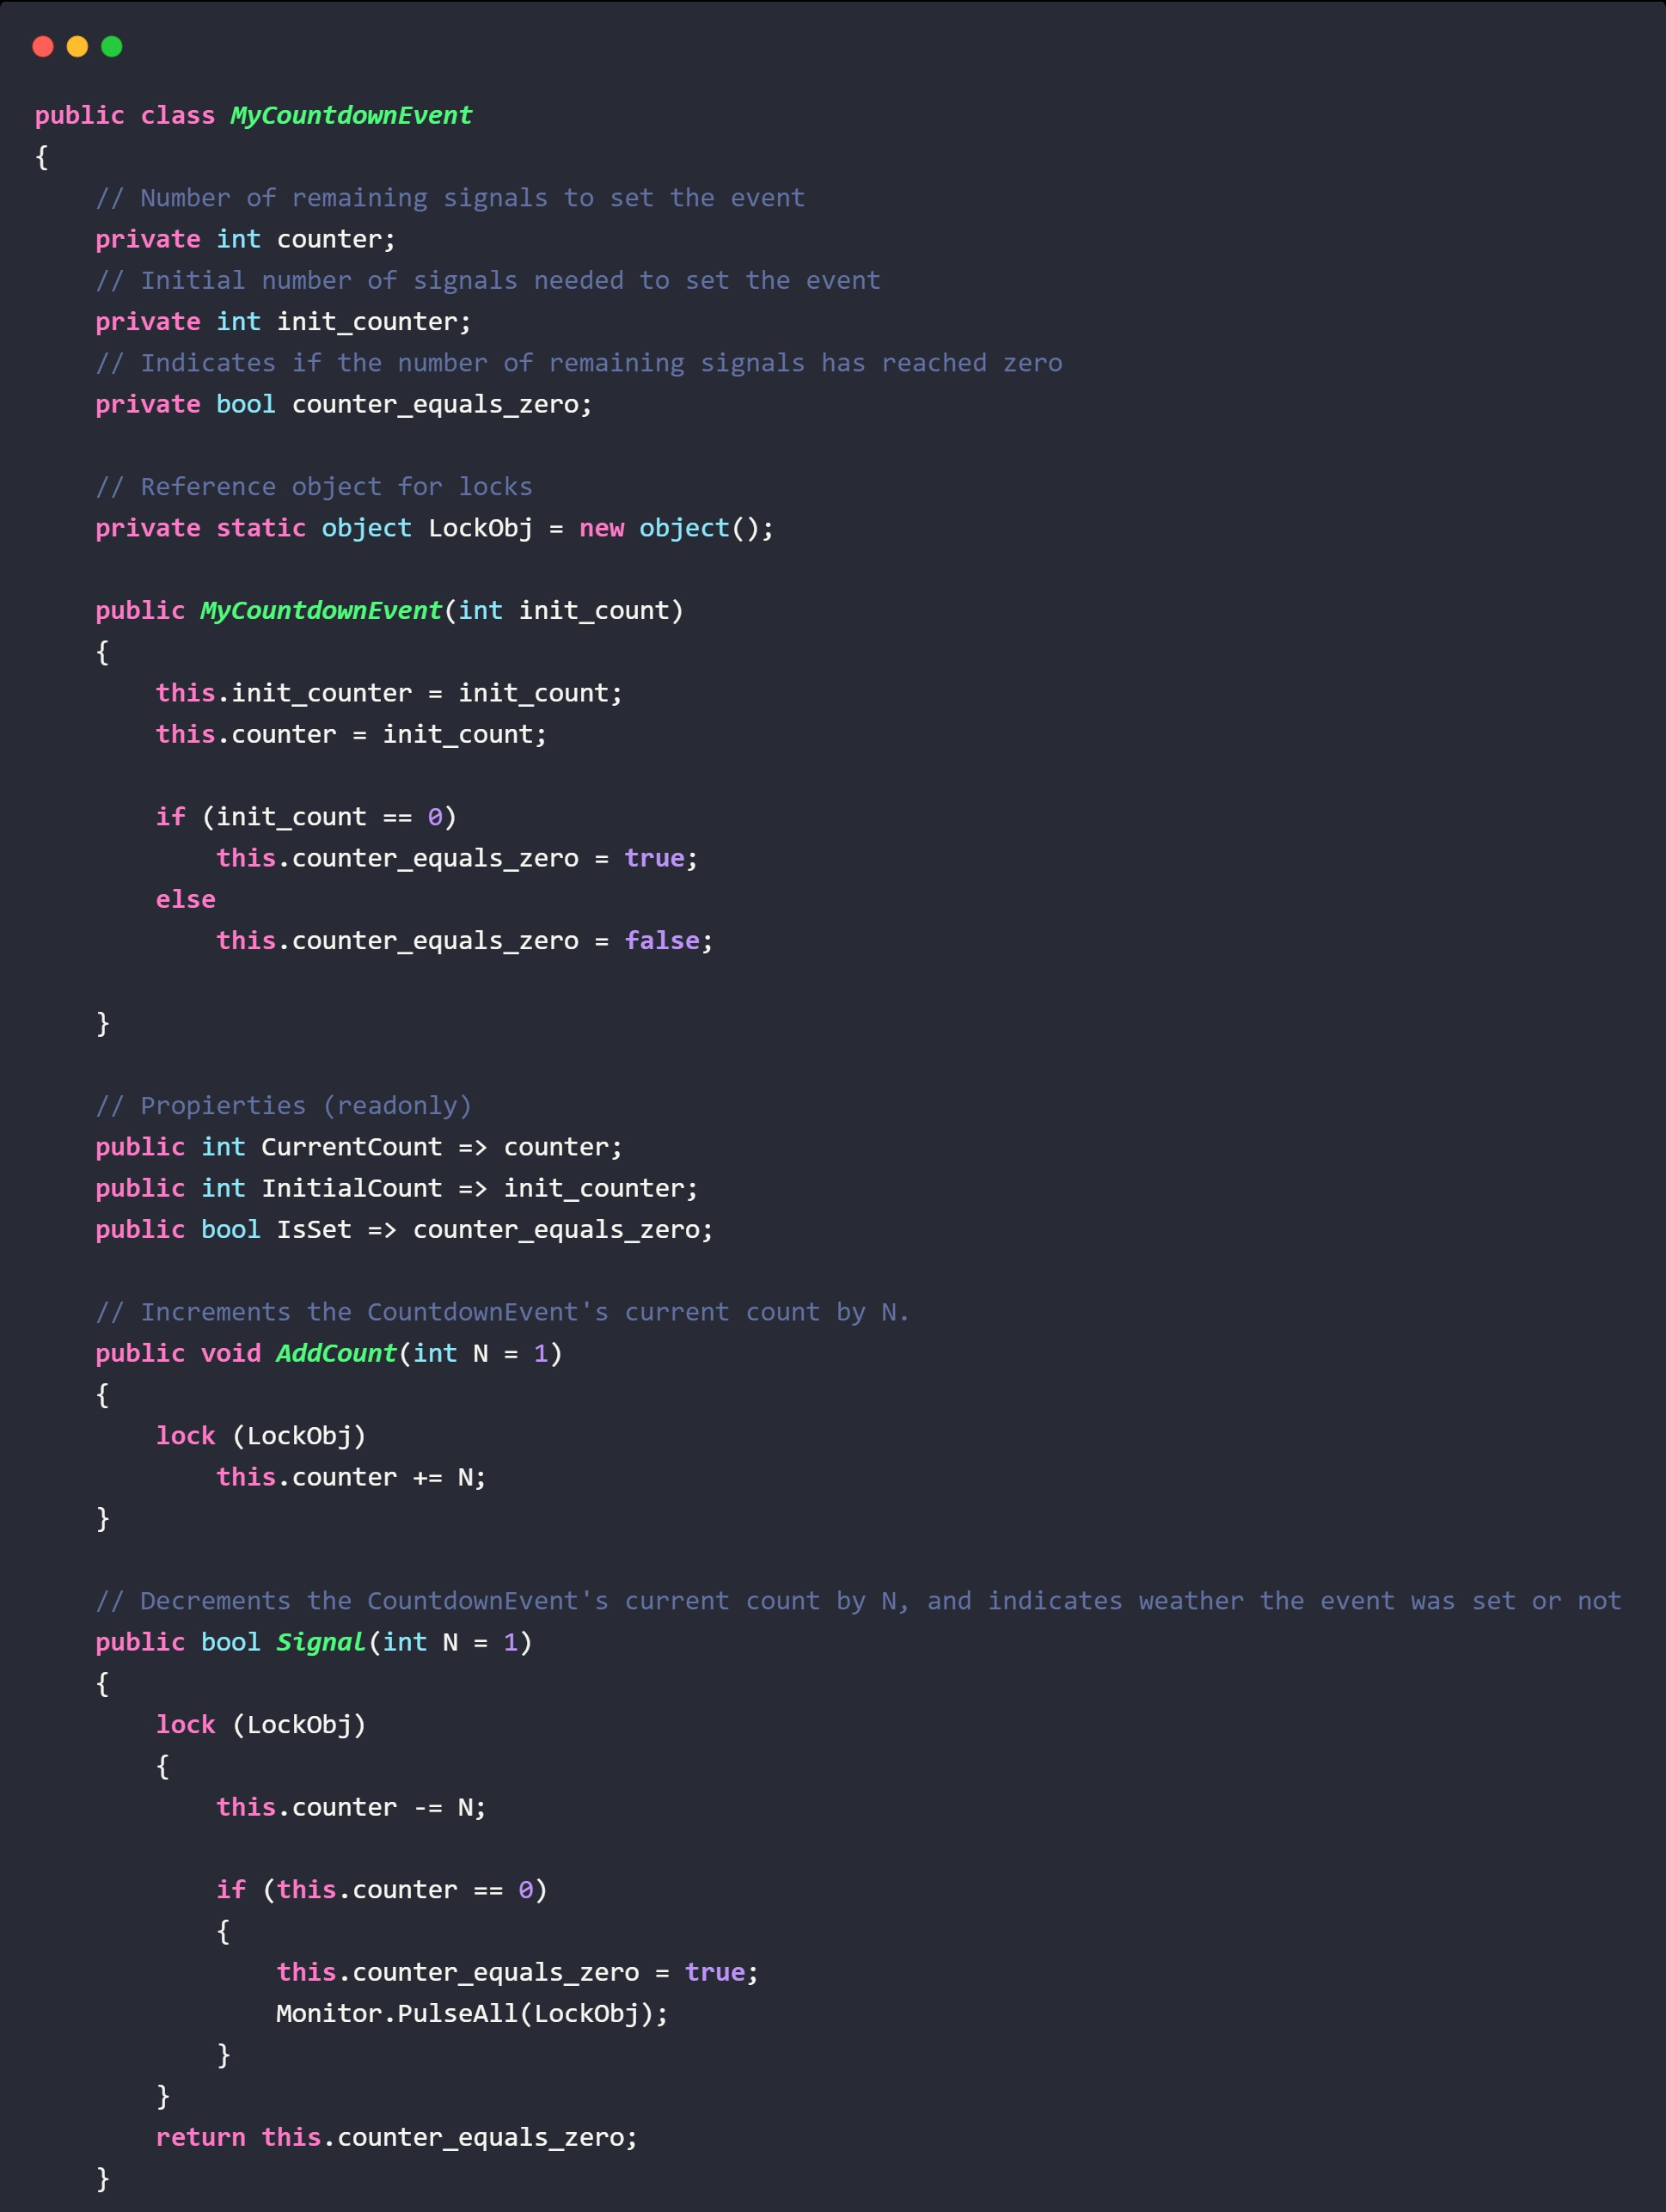
\includegraphics[width=15cm]{MyCountdownEvent1.jpg}
\end{center}

\begin{center}
	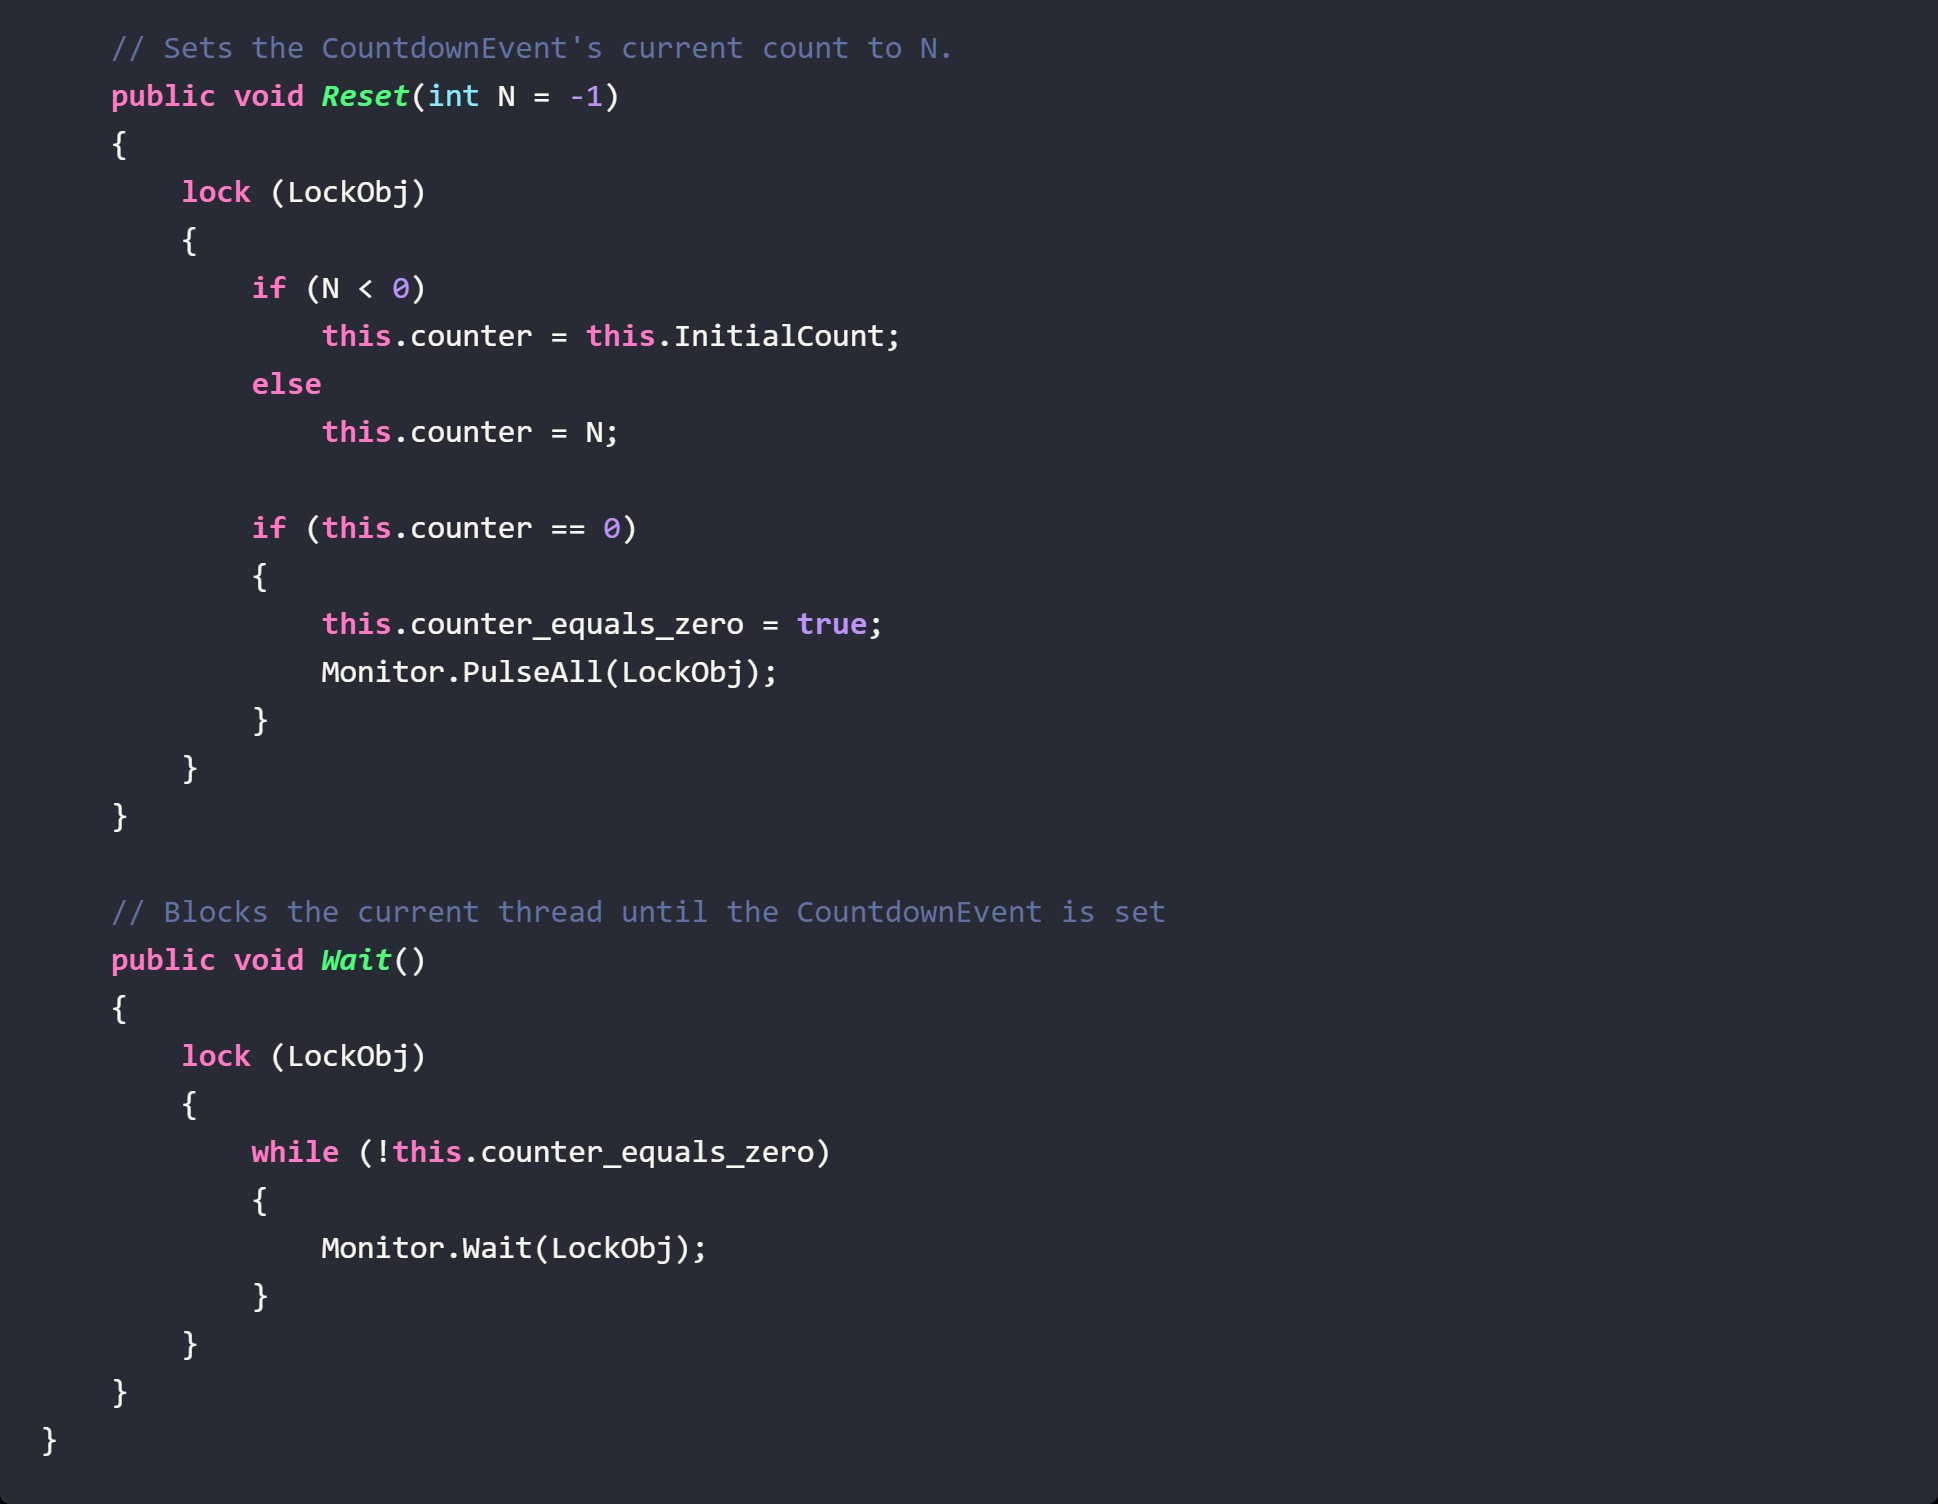
\includegraphics[width=15cm]{MyCountdownEvent2.jpg}
	
	\imgcaption{7}{Implementaci\'on de MyCountdownEvent utilizando Monitors}
\end{center}

\subsection{Concurrencia en Go}

Antes de entrar en detalles de como Go trata la concurrencia, es importante definir algunos conceptos importantes que ayuden a comprender mejor esta sección.

\subsubsection{Procesos, hebras y gorutinas en Go}

Un \textbf{proceso} es la representación en el SO (Sistema Operativo) de un \textbf{programa} en ejecución, mientras que un programa es un archivo binario en disco que contiene toda la información necesaria para crear un proceso en el SO. El archivo binario está escrito en un formato específico (ELF en Linux) y contiene todas las instrucciones que la CPU va a ejecutar, así como una plétora de otras secciones útiles. Ese programa se carga en memoria y las instrucciones se ejecutan, creando un proceso en ejecución. Así, un proceso lleva consigo recursos adicionales como memoria, descripciones de archivos abiertos y datos de usuario, así como otros tipos de recursos que se obtienen durante el tiempo de ejecución.

Un \textbf{hebra} es una entidad más pequeña y ligera que un proceso. Los procesos constan de una o más hebras que tienen su propio flujo de control y pila. Una forma rápida y simplista de diferenciar una hebra de un proceso es considerar un proceso como el archivo binario en ejecución y una hebra como un subconjunto de un proceso.

Una \textbf{gorutina} es la entidad Go mínima que puede ser ejecutada concurrentemente. El uso de la palabra mínima es muy importante aquí, ya que las gorutinas no son entidades autónomas como los procesos UNIX, las gorutinas viven en hebras del SO que viven a su vez en procesos del SO. Lo bueno es que las gorutinas son más ligeras que las hebras, que, a su vez, son más ligeras que los procesos, ejecutar miles o cientos de miles de gorutinas en una sola máquina no es un problema. Entre las razones por las que las gorutinas son más ligeras que los hilos está que tienen una pila más pequeña que puede crecer, tienen un tiempo de arranque más rápido y pueden comunicarse entre sí a través de canales con baja latencia. Por defecto, cada gorutina reserva 2Kb de memoria al inicializarse y a medida que se va necesitando más, va pidiendo.

En la práctica, esto significa que un proceso puede tener múltiples hebras así como muchas gorutinas, mientras que una gorutina necesita el entorno de un proceso para existir. Así, para crear una gorutina, necesitas tener un proceso con al menos una hebra. El SO se encarga del manejo de procesos y hebras, mientras que Go crea las hebras necesarias y el desarrollador crea el número deseado de gorutinas.

\subsubsection{Planificador de Go}

El planificador (scheduler) del núcleo del SO es responsable de la ejecución de las hebras de un programa. Del mismo modo, el \texttt{runtime} de Go tiene su propio planificador, que es responsable de la ejecución de las gorutinas utilizando una técnica conocida como \textbf{M:N scheduling}, donde M gorutinas se ejecutan utilizando N hebras del SO usando multiplexación. El planificador de Go es el componente de Go responsable de la forma y el orden en que se ejecutan las gorutinas de un programa Go. Esto hace que el planificador de Go sea una parte realmente importante del lenguaje de programación Go. 

Para encontrar más información acerca del planificador de Go, se recomiendo consultar la siguiente bibliografía \cite{scheduler}.

\subsection{Propuesta de Go para la sincronización de gorutinas}

En Go, se abordan dos enfoques distintos para lograr la sincronización de gorutinas, el primero es el enfoque clásica que es compartir datos a través de la memoria compartida, y el segundo enfoque e innovador de Go, es el de compartir memoria a través de los datos.

\subsection{ Sincronización a bajo nivel (paquete sync) }

Este es el enfoque clásico haciendo uso de la memoria compartida. Es importante aclarar que solo se presentan en este trabajo algunas de las formas más usadas de tratar la concurrencia usando este enfoque en Go, pero existen otras.

\subsubsection{WaitGroup}

En ocasiones es conveniente dividir el flujo de ejecución de un programa en pequeñas subrutinas que deben ser ejecutadas de manera concurrente, pero que tienen una lógica que las agrupa y no tiene sentido seguir ejecutando el programa hasta que todas por independiente lleguen a un estado exitoso.

Para esto se crea la estructura \emph{WaitGroup} que tiene 3 métodos principales, el primero \emph{Add(count int)} que recibe un entero que indica el incremento del contador en el grupo, \emph{Done()} que indica que una subrutina del grupo fue terminada de ejecutar con éxito (nótese que una llamada a \emph{Done()} es equivalente a \emph{Add(-1)}), y por último pero no menos importante la función \emph{Wait()} que marca un punto de bloqueo, y hasta que todas las subrutinas del grupo no se hayan ejecutado correctamente y el contador haya disminuido a 0, no continua la ejecución del programa.

Un ejemplo del uso de la estructura \emph{WaitGroup} se encuentra en el archivo \textit{waitGroup.go}. 

\subsubsection{Mutex}

Al igual que otros lenguajes de programación, \emph{Mutex} brinda un mecanismo de bloqueo con el objetivo de proteger las zonas críticas del código. Posee una función \emph{Lock()} que sirve para indicar que a partir de esa línea de código está bloqueado el acceso desde cualquier gorutina diferente a la que se le hace el llamado. Y tiene un método \emph{Unlock()} que indica la finalización de zona crítica y con esto el desbloqueo de los recursos.

Véase un ejemplo en el archivo \textit{mutex.go}, que es una pequeña modelación de un sistema de votación electrónico. Imagínese que dos votantes desean votar por el mismo candidato y estos acceden al recurso de la cantidad de votos en el mismo instante de tiempo, de \textit{N} votos que tenía el candidato tendrá luego de incrementar el valor en ambas gorutinas \textit{N+1} votos, lo cuál es incorrecto puesto que debería incrementar 2 votaciones. La solución a esto es bloquear la zona de incrementar la cantidad de votaciones. 

\subsubsection{RWMutex}

\emph{Mutex} resuelve el problema de proteger las secciones críticas del código, pero puede mejorarse aún más. El problema con el acceso a los recursos compartidos no es la lectura de estos, sino la escritura. \emph{RWMutex} permite diferenciar las zonas de bloqueo de escritura y de lectura.

Como la estructura \emph{RWMutex} está compuesta por \emph{Mutex}, los métodos \emph{Lock()} y \emph{Unlock()} se tratan de la misma forma, y se utilizan para indicar las zonas de escritura. La diferencia principal entre estas dos estructuras radica en que las zonas de lectura permiten ser accedidas desde distintas gorutinas, permitiendo así una mayor fluidez de su programa. Para indicar los límites de las zonas de lectura se utilizan los métodos \emph{RLock} y \emph{RUnlock}. Es importante mencionar, que la zona de escritura se considera desbloqueada si y solo si no hay ninguna gorutina escribiendo, ni ninguna leyendo; y una zona de lectura se considera desbloqueada si no hay ninguna gorutina escribiendo.

Se propone analizar el ejemplo práctico para entender estos conceptos. El problema consiste en tener una llave privada que se utiliza para firmar operaciones que realizan llamados a servicios \textit{gRPC}. Cada llamado a un servicio toma tiempo de espera determinado. Dicha llave privada se cambia con frecuencia, con el objetivo de evitar que sea robada fácilmente. 

Nótese que cuando se está cambiando la llave privada, ninguna gorutina puede estar accediendo a dicho recurso. En el momento que se desee acceder a un servicio, y se está escribiendo en ese instante, se bloquea la gorutina y espera a que se termine de escribir; una vez que esto pase, se permite el paso a la zona de lectura a todas aquellas gorutinas que quieren acceder a un servicio. (piense que sucedería si se abordara el enfoque clásico de Mutex, cuánto tiempo demoraría en salir del cuello de botella) 

Se deja el código fuente con el ejemplo, en el archivo \textit{rwMutex.go}. Debe tenerse en cuenta que la estructura RWMutex tiene otros métodos, pero por su poco uso cotidiano no se considera necesario abordarlos en este informe.

\subsubsection{Once}

La primitiva de bajo nivel \emph{Once} tiene como objetivo ejecutar una función una única vez. Esta tiene un método \emph{Do()} que es el que se encarga de asegurar que una función se ejecute a lo sumo una vez utilizando ese objeto \emph{Once}, o sea, no significa que la función no se pueda ejecutar varias veces, sí puede hacerlo, pero utilizando la función \emph{Do()} de una instancia específica de la estructura \emph{Once} solo se puede ejecutar una vez. Verifique por ud mismo que dados dos objetos \emph{Once} es posible ejecutar una función 2 veces, una vez por cada objeto.

Se deja una ejemplo en el archivo \textit{once.go}, donde se quieren hacer operaciones con objetos en una base de datos, pero se sabe que cada fila en una base de datos necesita tener un identificador único, por tanto cada vez que se quiere hacer una operación en la base de datos con un objeto de tipo Persona, se asegura primero que se haya inicializado antes, dándole un identificador único a cada objeto, y luego se hacen las operaciones que se deseen en la base de datos.

\subsection{Sincronización a alto nivel.}

En los sistemas UNIX, existe un concepto llamado Pipeline, su traducción al español viene siendo tubería, o cualquier sinónimo que haga referencia a un conducto de comunicación. En dichos sistemas, las tuberías se utilizan para la sincronización de procesos a bajo nivel, proveendo un forma efectiva de comunicación.

En Go no hablamos de procesos, ni de hebras, quien se encarga de lidiar con estas son el SO y el planificador de Go. El desarrollador de Go, de lo que entiende es de gorutinas, que vienen siendo un análogo a una hebra en un SO, pero no son lo mismo (leer sección \emph{VI.1}). Entonces para la comunicación de estas, además de tener el enfoque clásico de sincronizacón en la concurrencia, se crea un nuevo enfoque el cual se basa en compartir memoria a través de los datos. 

Go logra esta forma de sincronización creando un tipo en el lenguaje llamado \textbf{chan} (o canal), que es el encargado de transferir información entre una gorutina y otra. Los canales en Go funcionan de manera muy similar a como funcionan las tuberías en los sistemas UNIX. 

\subsubsection{Canales sin búfer}

En un servidor web, cuando se tiene abierto un socket esperando peticiones, hasta que el cliente no intente establecer una comunicación con el servidor y este lo acepte no comienza el intercambio de información. Exactamente esto pasa con la transferencia de datos a través de canales sin búfer. Como no tiene espacio para guardar información, bloquea el flujo de ejecución de una gorutina hasta que estén ambas partes, quien envía y quien lee la información.

Para la creación de un canal, se utiliza la función built-in \textbf{make(chan Type, capacity int)}. Crear un canal sin búfer se puede hacer de dos formas, \textit{make(chan Type)} o \textit{make(chan Type, 0)}. Note que para la creación de un canal es necesario especificar el tipo de datos que se desean transferir por él.

Se deja un ejemplo en el archivo \textit{unbufferedChan.go}. Note como la gorutina principal no escribe en el canal hasta que la gorutina de lectura del canal no está lista para recibir la información. 

\subsubsection{Canales con búfer}

A diferencia de los canales sin búfer (también pueden considerarse canales con búfer de capacidad 0), estos contienen una pila FIFO para el almacenamiento de información. La capacidad de esta pila es definida en el momento de creación del canal. En el momento en que la pila esté llena, se bloquea cualquier intento de escritura en el canal, hasta que haya espacio disponible.

Apóyese en el ejemplo que se encuentra en \textit{bufferedChan.go}, el cual es similar al ejemplo anterior, pero a diferencia de que el canal tiene un buffer de capacidad 5. Se escribe hasta repletar su capacidad y luego se va leyendo del canal, uno a uno, con intervalos de 1 segundo entre una lectura y la siguiente; con esto se libera espacio, por tanto se puede volver a escribir, esto llenaría de nuevo el canal, luego se lee, se libera, y así sucesivamente. 

\subsubsection{Select}

La estructura \emph{select-cases} permite leer o escribir de varios canales al mismo tiempo. En caso de que hayan varias opciones de lectura y/o escritura en el mismo instante, Go escoge una al azar y es la que se selecciona. Esta estructura es muy parecida al \textit{switch-case} que existe en muchos lenguajes de programación.

Se deja un ejemplo en \textit{select.go} del uso de esta estructura. El ejemplo consiste en simular el envío de información entre un servidor y dos clientes que se conectan a él, y le envían información, con la restricción de que el servidor no puede exceder un límite de tiempo de espera prefijado (en este ejemplo es 40ms). En caso de ser excedido este límite de tiempo se corta la comunicación entre clientes-servidor y se da por concluído el envío de información. 

Este patrón de diseño para controlar un límite de tiempo esperando un recurso, se conoce en la literatura como \emph{Timing out, moving on}, y existen varias formas de resolver esta situación. La utilizada en este ejemplo es usando la función \emph{time.After(timeout int)} que dado un número que equivale al tiempo de espera, devuelve un canal que dará un ping luego de transcurrido este tiempo. Entonces, si se está esperando por la lectura de varios canales incluído este último, luego de pasar el tiempo predefinido y no se ha escrito en ninguno de los otros canales, se lee de este y se ejecuta la acción que se desee. En este ejemplo, las acciones deseadas son notificar a cada uno de los clientes que el servidor va a dejar de recibir información y luego se cierra el servidor. 

La vía de notificación del servidor al cliente es el mismo canal por el que el cliente le enviaba información al servidor. Esto trae consigo algunas complicaciones por el lado del cliente, como por ejemplo saber diferenciar entre el signal que le envío el servidor para avisarle de que no recibirá más información, y la propia información que le enviaba él mismo al servidor. Esto lo puede resolver el servidor enviando un valor distintivo al que envía el cliente (en este caso -1); y otra forma de resolverlo es hacer el canal sin búfer, lo cual traería otras complicaciones. 

La solución dada sigue siendo una solución parcial al problema, da error en el caso en que el servidor esté notificando a los clientes de que dejará de recibir información, y la gorutina de un cliente se haya quedado en la instrucción a punto de enviar la información, al intentar enviarla se quedará esperando a que se libere espacio del canal, pero esto nunca sucede. Por este mismo motivo falla también la solución que se propuso arriba de utilizar un canal sin búfer. Aunque todos estos problemas se pudieran resolver dándole mayor capacidad al canal, no se hizo. Más adelante se mostrará una forma más elegante de resolver estos problema.

\subsubsection{Canales de canales}

Como se había mencionado anteriormente los canales son una estructura capaz de transferir instancias de un tipo definido. Resulta que los canales también son un tipo en Go, por tanto se permite crear canales del estilo \emph{chan chan <type>}. A continuación se presenta un ejemplo (\textit{channelChan.go}) donde se evidencia la utilidad de un tipo de esta forma.

Extendiendo un poco el ejemplo presentado en la sección anterior, ahora se quiere tener un servidor esperando peticiones de clientes para conectarse a él. Luego de aceptada la conexión con el servidor, este envía al cliente un \emph{chan string} para intercambiar información con él, esto es lo que vendría siendo habilitarle un puerto para la comunicación. Este envío de un medio para la comunicación se hace a través de un \emph{chan chan string}.

\subsubsection{Canales con restricción}

La solución anterior aún está defectuosa, se propone analizar al detalle los motivos que provocan estos \texttt{deadlocks}, pero se puede afirmar que el motivo principal por lo que son provocados es que un mismo canal está asumiendo varias funcionalidades y se permite tanto escribir como leer desde cualquier gorutina, lo cual trae fuertes conflictos porque el desarrollador no es quien controla el orden en que se ejecutan estas gorutinas. 

Para desacoplar las funcionalidades de cada canal, obtener mayor expresividad y lograr un jerarquía más robusta ante posibles fallos futuros se introduce el concepto de canal con restricción. Un canal con restricción no es más que un canal unidireccional, donde solamente se puede escribir o leer, una de dos. La sintaxis para lograr esto es \textit{chan<- Type} para indicar que el canal es de solo escritura y \textit{<-chan} de solo lectura.

A continuación se presenta un ejemplo \textit{restrictedChan.go} que da una solución final al problema planteado.

\subsection{Problema de los 5 Fil\'osofos}

El problema presentado en esta secci\'on es un problema cl\'asico para ejemplificar los problemas de sincronizaci\'on,  el cual fue tomado de (\cite[Ep\'igrafe 17.7.2.1]{katrip}).

\textbf{Descripci\'on:} Cinco fil\'osofos se pasan la vida comiendo y pensando, sentados en una mesa circular con un taz\'on com\'un en el centro que contiene ``infinitos" espaguetis y con un tenedor colocado entre cada par de fil\'osofos. Cada fil\'osofo alterna a su antojo el comer y el pensar, sin comunicarse con los dem\'as. Para comer, cada fil\'osofo necesita de los dos tenedores (el que tiene a su izquierda y el que tiene a su derecha) por lo que puede ocurrir que tome uno de los dos tenedores y tenga que esperar por el otro que est\'a ocupado por su vecino. Al terminar de comer el fil\'osofo debe colocar de vuelta los tenedores sobre la mesa. Puede ocurrir una situaci\'on en que cada filo\'osofo tenga ocupado el tenedor a su izquierda y al querer tomar el tenedor a su derecha este est\'e ocupado por el fil\'osofo a su derecha quien tambi\'en est\'a en la misma situaci\'on y, as\'i, de modo circular. Entonces todos est\'an bloqueados sin poder comer por falta de un tenedor.

\textbf{Problema:} Dise\~nar un m\'etodo con el cual los fil\'osofos puedan alternar entre comer y pensar eternamente, sin previo conocimiento de cu\'ando los otros fil\'osofos desean comer y, claro, sin tener que aumentar la cantidad de tenedores porque es obvio que si cada uno tiene dos tenedores no habr\'ia problema.

\subsubsection{Soluci\'on en C\#}

En \cite[Ep\'igrafe 17.7.2.2]{katrib} podemos encontrar una soluci\'on parcial al problema. La misma consiste en usar un mediador (mesero) que determine en cada momento qui\'en puede o no usar los tenedores seg\'un los soliciten. De esta forma se elimina la posibilidad de interbloqueo y por tanto que el programa quede esperando infinitamente. Sin embarago, se dice que es una soluci\'on parcial ya que no elimina la posibilidad de muerte por inanici\'on. La propuesta dada consiste en que solo un fil\'osofo pueda pedirle al mesero ambos tenedores, en cada momento. Sin embargo la decisi\'on de qu\'e fil\'osofo es atendido primero queda en manos del sistema operativo, y no sabemos como se comporta este, pudiendo darse el caso en que deje a uno de los fil\'osofos esperando sin ser atendido nunca, o relativamente pocas veces.

Para evitar ese problema en este trabajo se propuso contar con una cola en la que los fil\'osofos se van colocando cuando necesitan comer. La idea es que cuando un fil\'osofo decida comer este revise la cola a ver si no hay nadie que quiera alguno de sus dos mismos tenedores (y que tendr\'ia por ende prioridad), as\'i como revisa a quienes est\'an comiendo para ver que no est\'en ya ocupados. En caso de que coger los tenedores sea consistente con lo anterior, este los toma y se sienta a comer. Si no, se coloca al final de la l\'inea. Por supuesto, mientras un fil\'osofo est\'a comiendo sus tenedores est\'an bloqueados para el resto. Cuando un fil\'osofo termina de comer este avisa al mesero qui\'en revisa la cola por si alguien estaba esperando por alguno de esos tenedores. La cola se revisa por orden de llegada (FIFO) y de este modo se garantiza que come primero siempre el que primero decidi\'o comer.\

Para implementar esto usaremos la clase \csl{Monitor}, qu\'e interactuar\'a sobre los objetos de tipo tenedor, para bloquearlos y desbloquearlos seg\'un se est\'en usando. Entonces cuando un fil\'osofo debe comenzar a comer, se revisa si los tenedores correspondientes no est\'an bloqueado (en uso) y si adem\'as la cantidad de gente en la cola esperando por cada uno de estos es cero. Si estas condiciones se cumplen se puede proceder a comer sin problemas, ya que no se afecta a m\'as nadie. Se bloquean entonces los dos tenedores que se usar\'an. Si este no es el caso entonces esta instancia de fil\'osofo se adiciona a la cola, y adem\'as se bloquea la ejecuci\'on de su hebra mediante \csl{Monitor.Wait}, mientras espera una se\~nal de \csl{Monitor} correspondiente al objeto \csl{Ticket} (campo de la clase \csl{Philosopher}).

Por otro lado tenemos en la hebra principal (disjunta de las 5 correspondientes a los fil\'osofos) un bucle infinito que en en cada iteraci\'on revisa la cola para darle los tenedores libres al que primero los necesite, haciendo \csl{Monitor.Pulse} a su \csl{Ticket} correspondiente. Sin embargo, si se hace esto consecutivamente se caer\'ia en un problema de interbloqueo. Adem\'as, es innecesario revisar la cola dos veces seguidas si no se han liberado tenedores nuevos. Entonces la ejecuci\'on de esta hebra queda bloqueada nuevamente por la clase \csl{Monitor}, aplicada sobre el objeto \csl{Waiter}, hasta que alg\'un fil\'osofo termine de comer y de la se\~nal de desbloqueo.

\begin{center}
	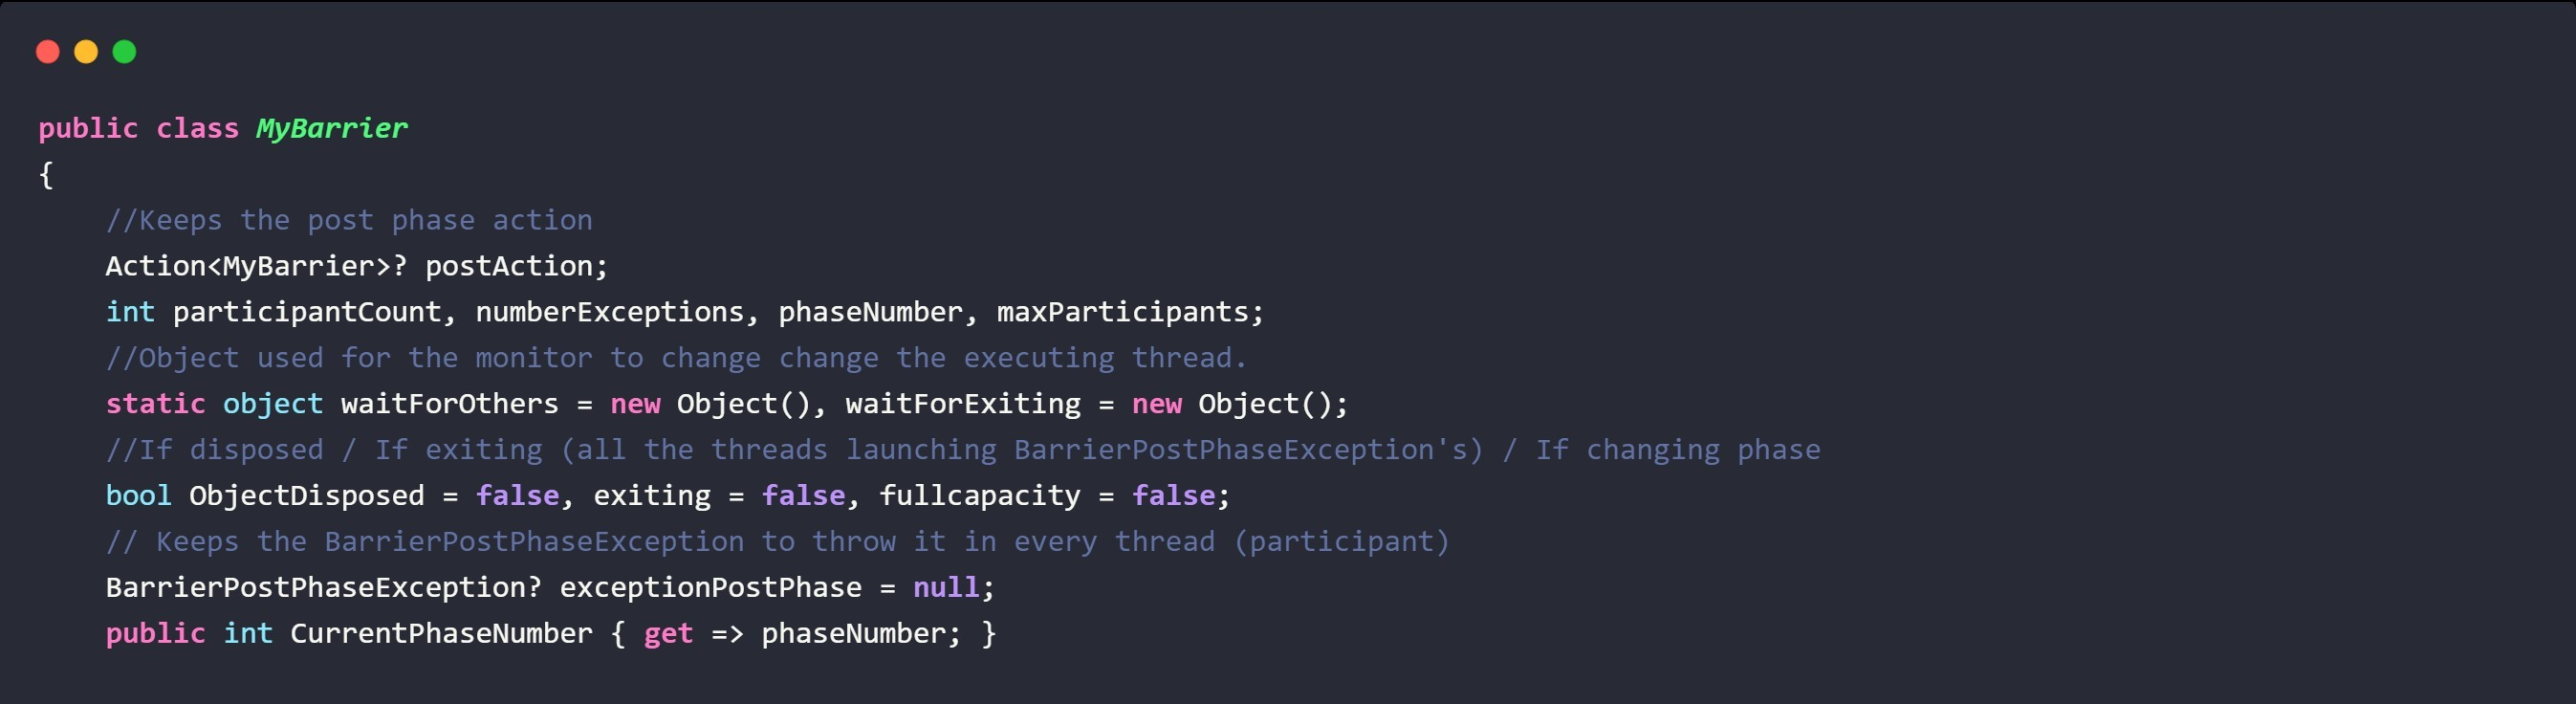
\includegraphics[width=15cm]{Philosopher_Live1.jpg}
\end{center}

\begin{center}
	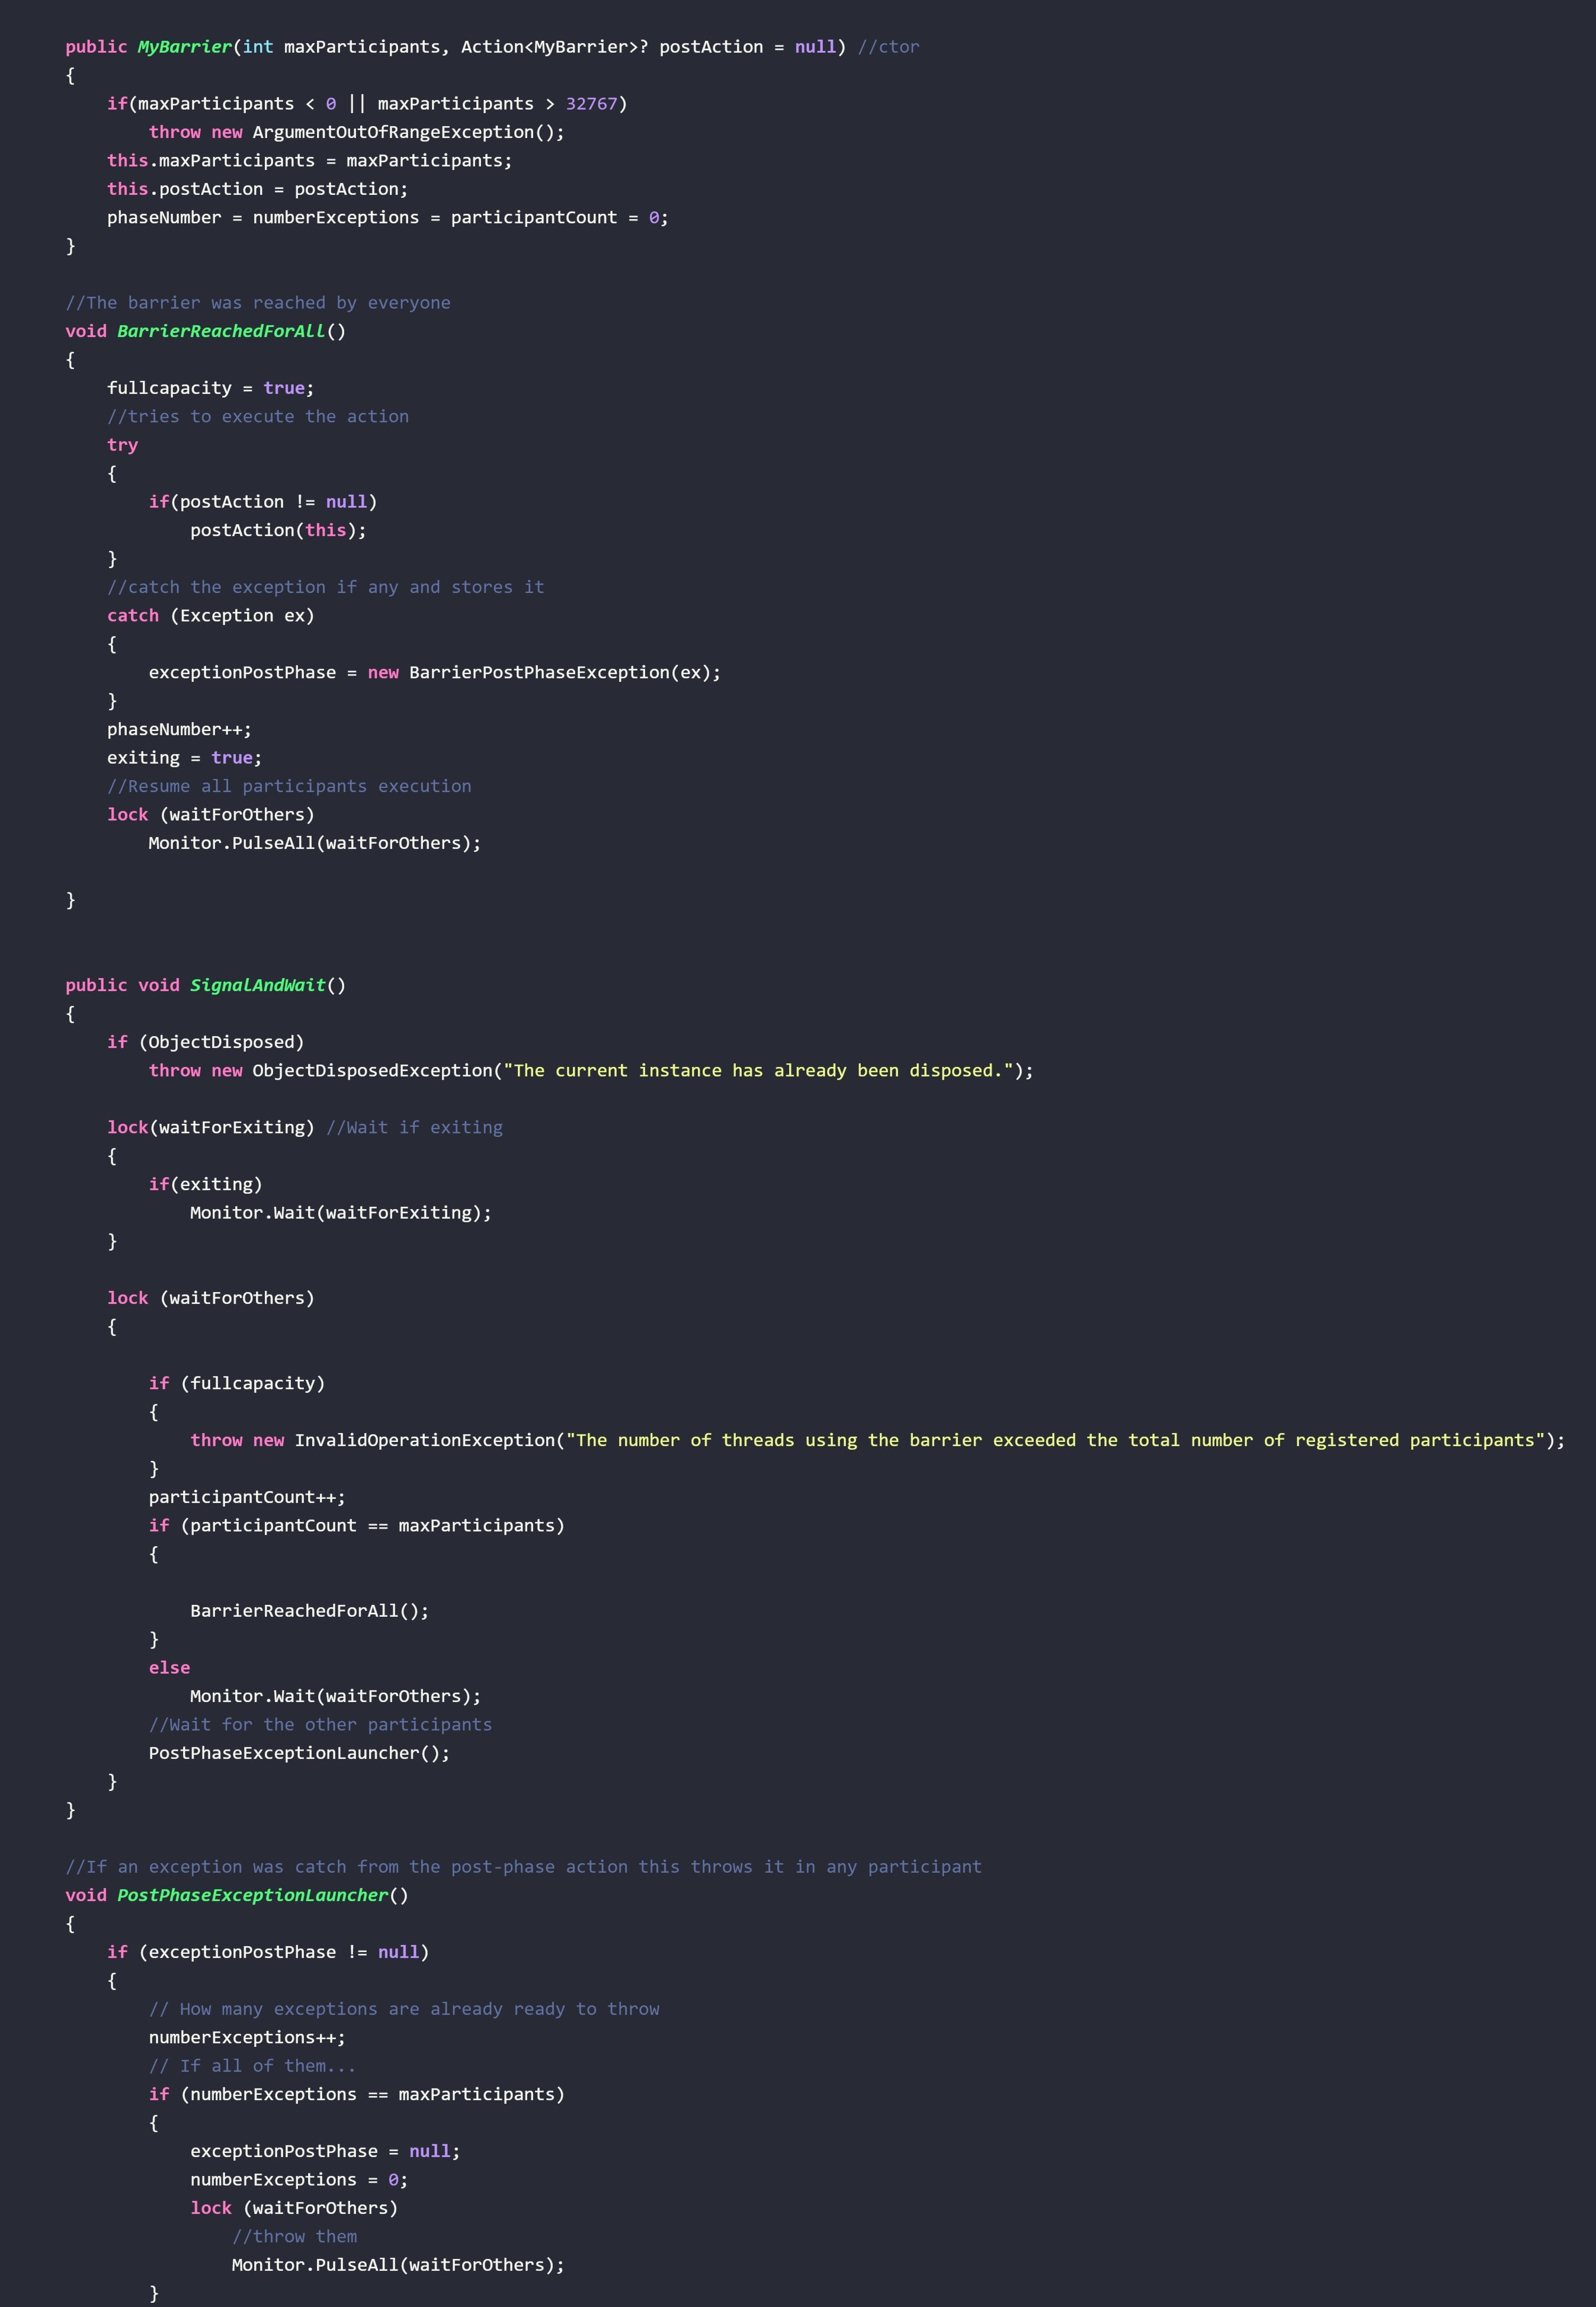
\includegraphics[width=15cm]{Philosopher_Live2.jpg}
\end{center}

\begin{center}
	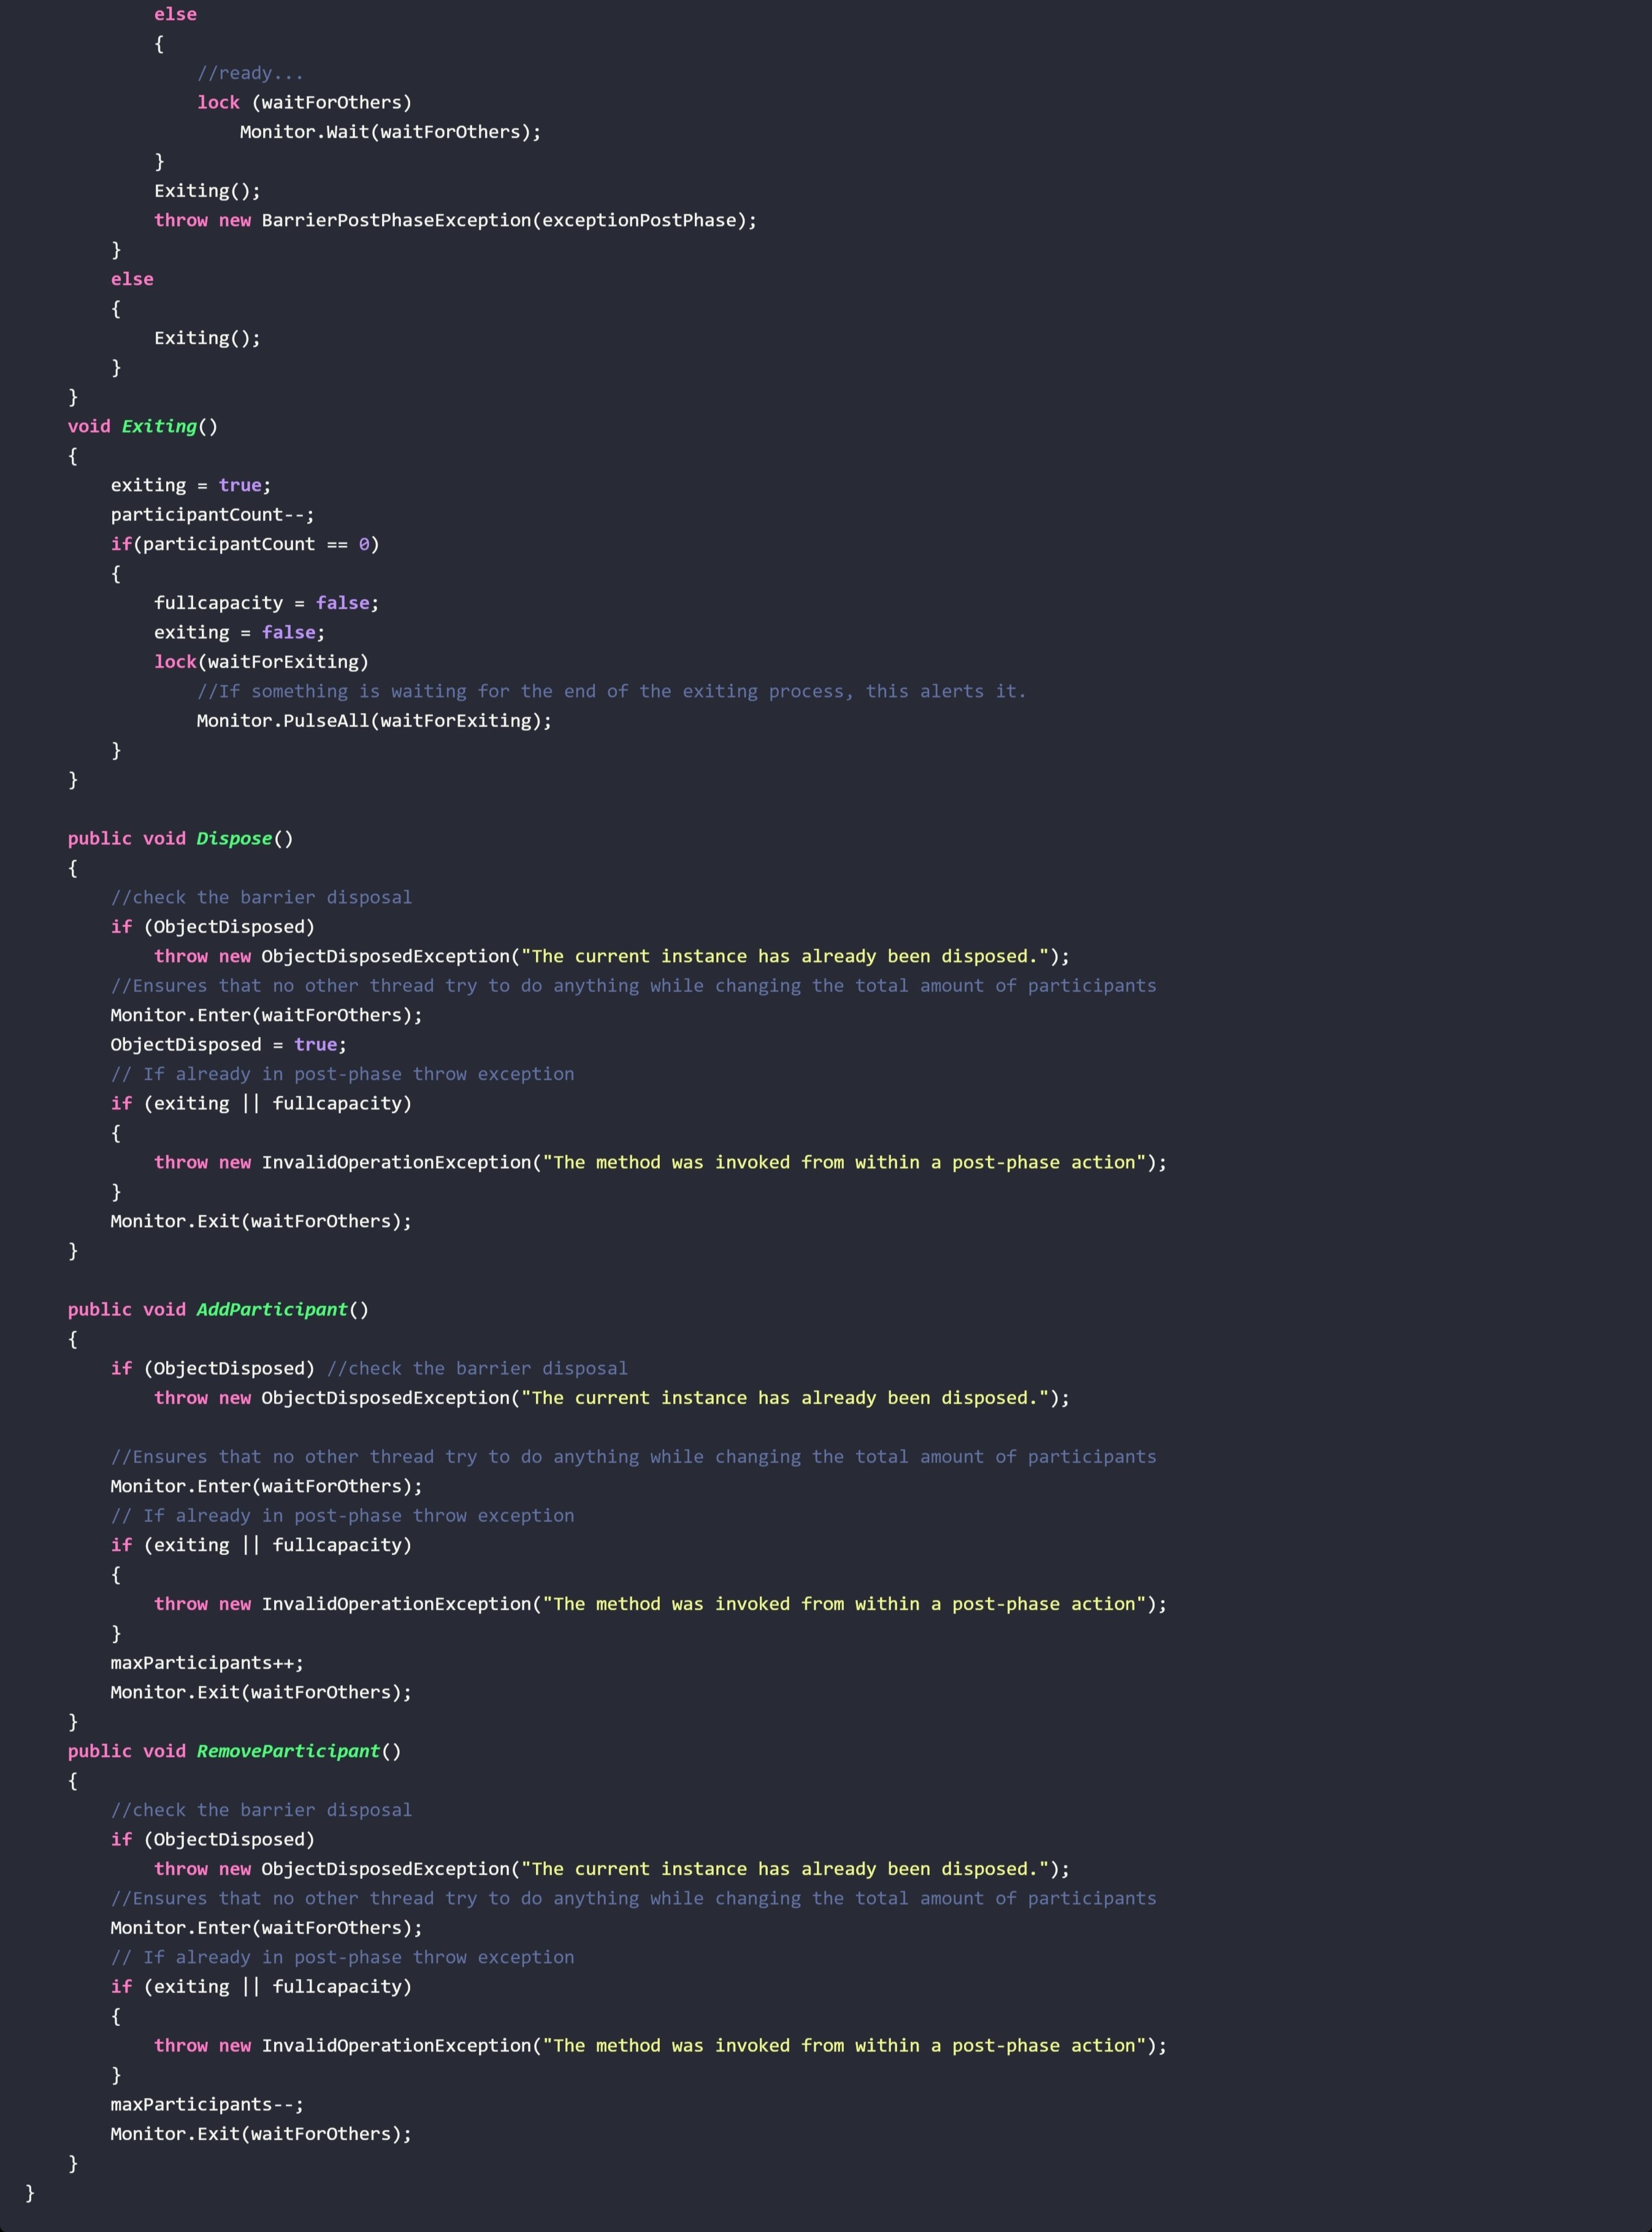
\includegraphics[width=15cm]{Philosopher_Live3.jpg}
	
	\imgcaption{8}{C\'odigo que muestra el comportamiento del fil\'osofo}
\end{center}

\begin{center}
	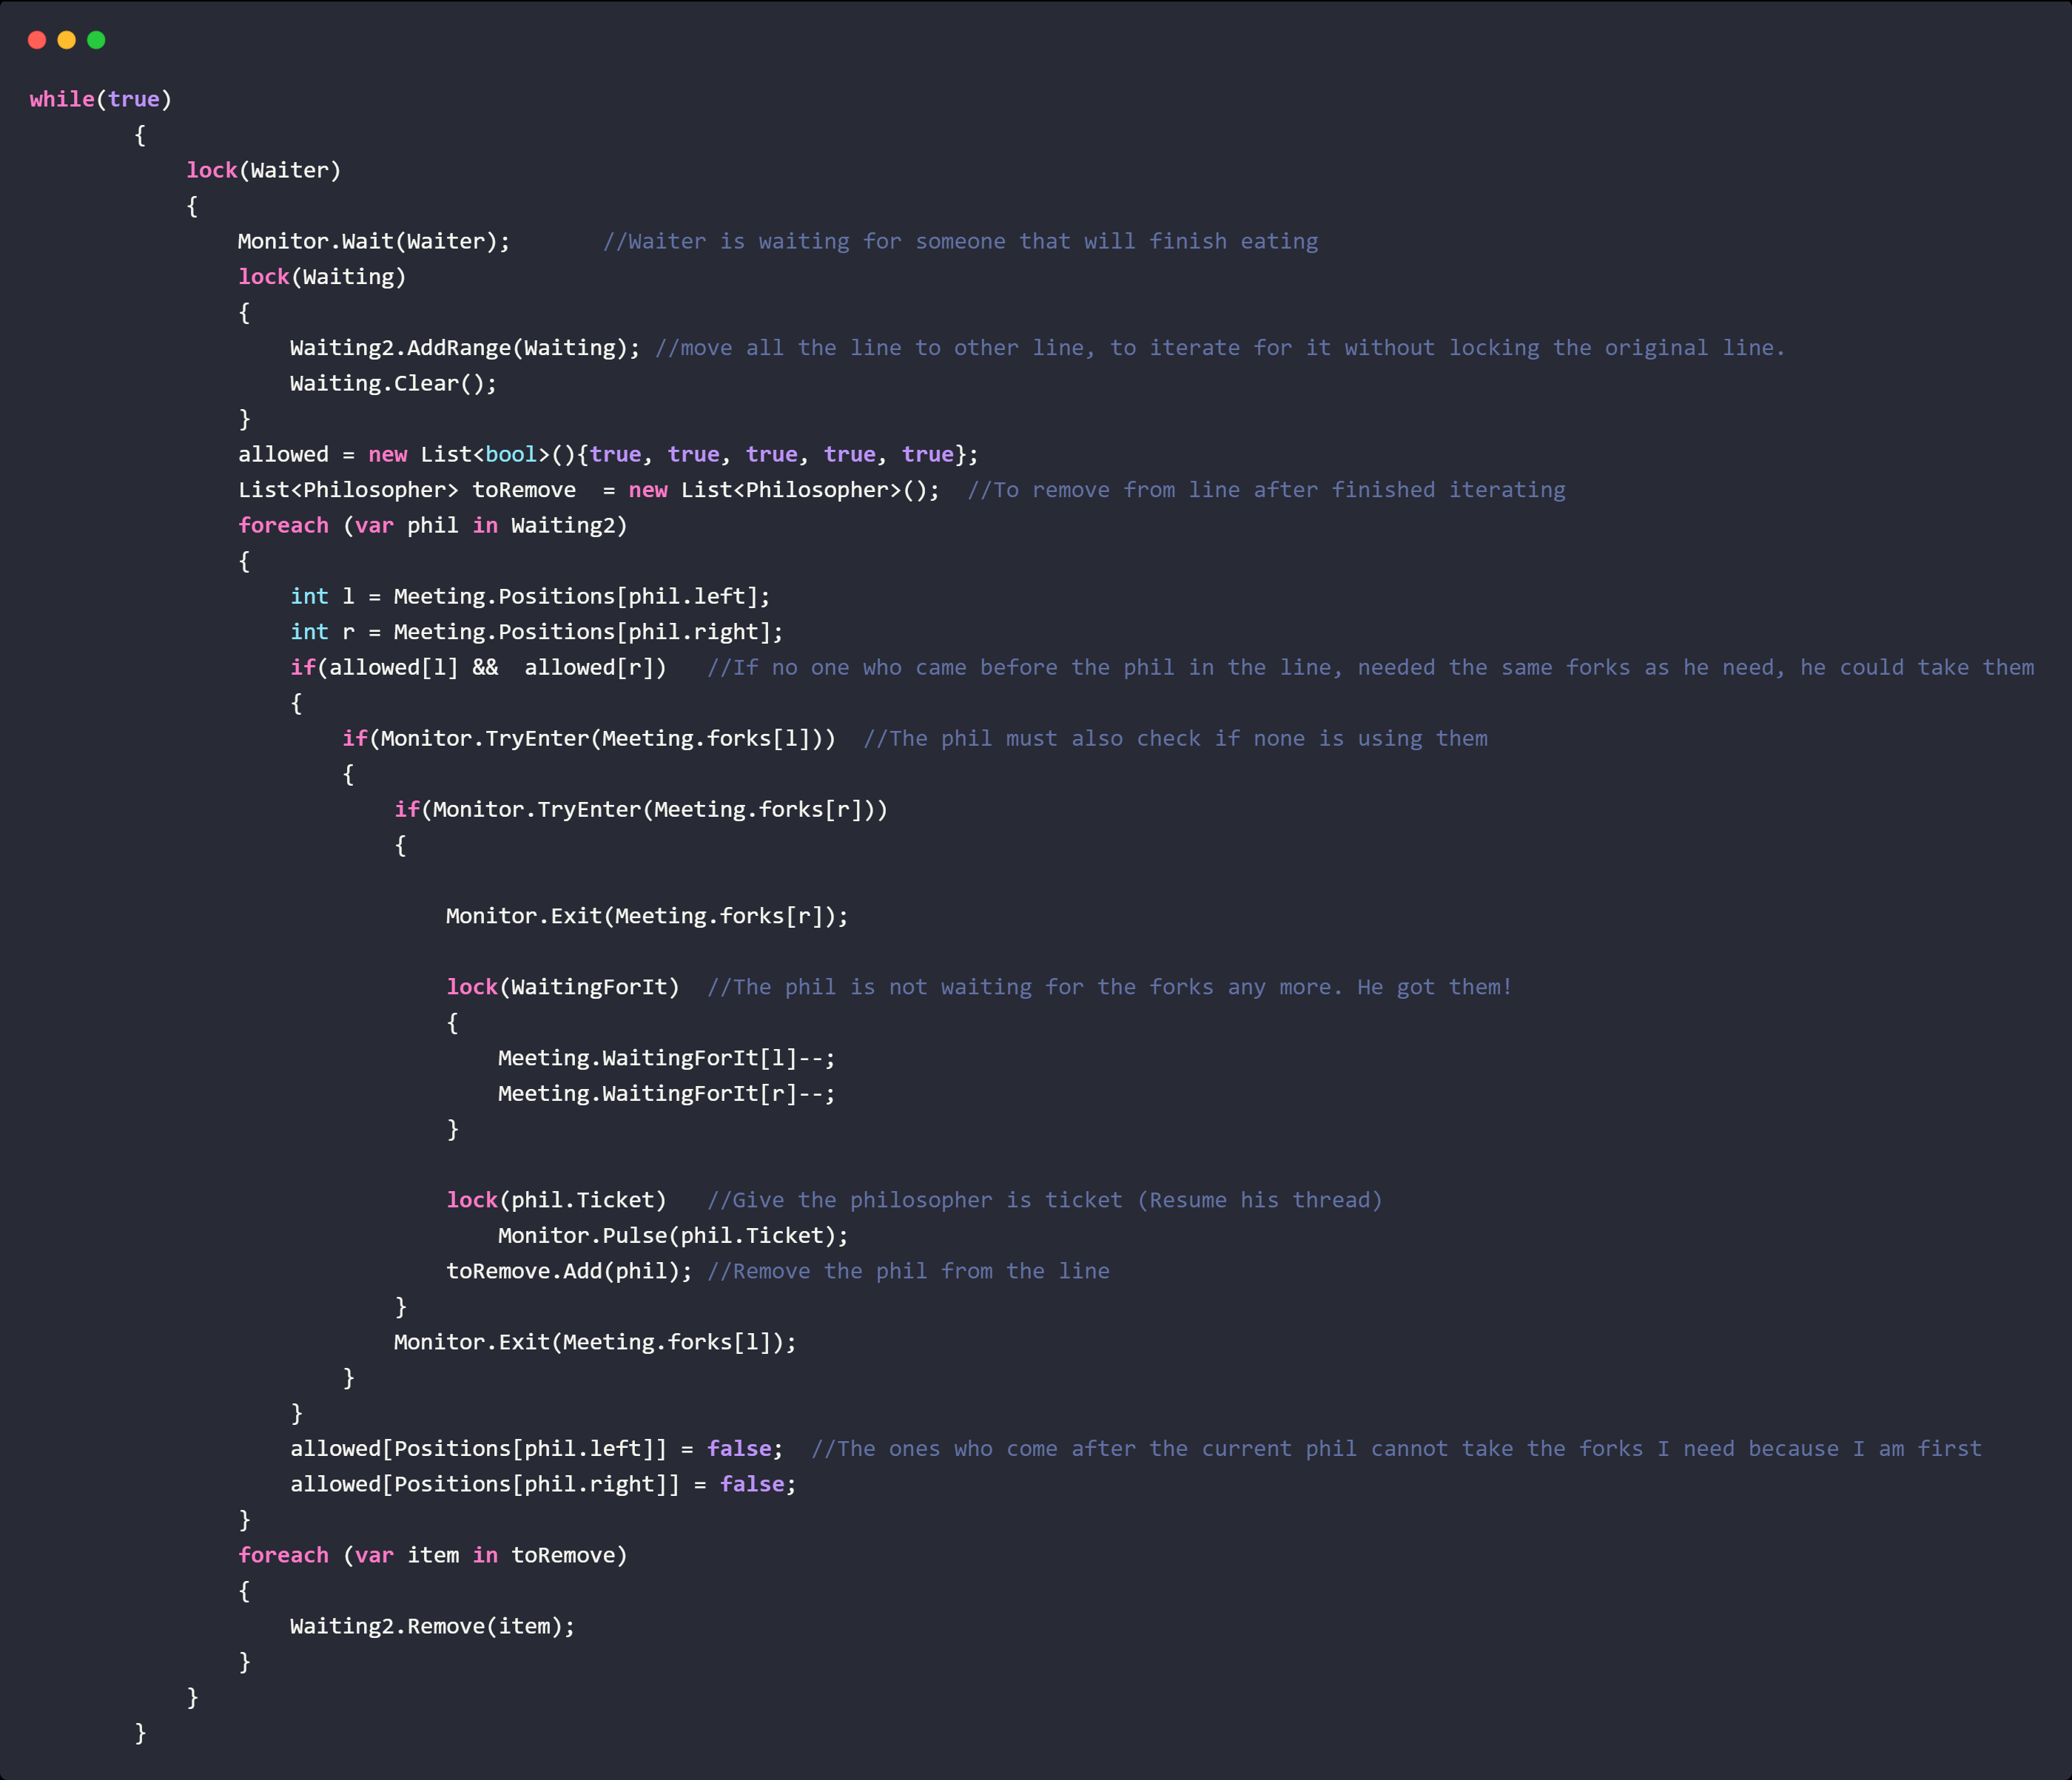
\includegraphics[width=15cm]{Philosopher_InfiniteLoop.jpg}
	
	\imgcaption{9}{C\'odigo que muestra el trabajo del mesero}
\end{center}

\subsubsection{Go}

La solución al problema de los filósofos implementada en Go no tiene un enfoque novedoso, parte de una idea sencilla e implementable en otros lenguajes de programación, a diferencia de que no permite escalar tan bien como en Go el número de filósofos sentados en la mesa. Esta solución permite ejecutar el problema de los \textit{N} filósofos con \textit{N = 700000} en una computadora de 8Gb de RAM.

La idea es que cada filósofo tenga una rutina de vida que se ejecuta de manera autónoma y repetitiva. Un filósofo lo primero que hace es pensar, luego intenta coger los cubiertos, en caso de no poder se pone a pensar nuevamente e intenta tomar los cubiertos más adelante. Luego de haber tomado los cubiertos come y finalmente suelta los cubiertos para que otros filósofos puedan utilizarlos.

Para coger los cubiertos el filósofo está dispuesto a esperar un tiempo \textit{T}, en caso de ser excedido ese tiempo y aún no haber tomado los dos cubiertos suelta el cubierto que tomó, en caso de haber tomado alguno, y se pone a pensar hasta que vuelve a intentar tomar los cubiertos.

Sobre los detalles de implementación en Go, los tenedores se modelaron como canales de capacidad 1 que solamente tienen acceso los filósofos que está sentados alrededor de estos. Si el canal está lleno significa que el tenedor está libre, en caso contrario que está siendo usado. Otro detalle de implementación importante es la simulación del ciclo de vida de cada filósofo de manera autónoma, esto se logra utilizando una gorutina por cada filósofo.

\subsubsection{Comparaci\'on}

El propuesta de Go para la concurrencia es mucho más rica en posibilidades respecto a la de C#, ya que aborda la sincronización desde dos enfoques distintos, compartir datos a través de la memoria compartida (la clásica implementada en muchos lenguajes de programación), y compartir memoria a través de los datos. Además de esto, la eficiencia de las gorutinas en Go permite que problemas como el propuesto anteriormente escalen a números realmente elevados.

\begin{thebibliography}
	a
	\bibitem{katrib} Miguel Katrib. \emph{Empezar a programar. Un enfoque multiparadigma con C\#}. 
	Editorial UH.
	2020.
	La Habana.
	\bibitem{microsoft} \href{https://learn.microsoft.com/en-us/dotnet/api/system.threading?view=net-7.0}{Microsoft Learn: System.Threading Namespace in .NET}
        \bibitem{scheduler} \href{https://morsmachine.dk/go-scheduler}{Go scheduler}
        \bibitem{mastering-go} Mihalis Tsoukalos. \emph{Mastering Go. Third Edition}, Packt.
\end{thebibliography}

\end{document}


